%\documentclass[a4paper,11pt]{article}%Schriftgröße
\documentclass[a4paper,12pt]{report}%Schriftgröße
\usepackage[T1]{fontenc} 
\usepackage[utf8]{inputenc}
\usepackage[english]{babel}%Veröffentlichungssprache

\usepackage{graphicx}
\usepackage{ragged2e}
\usepackage{amsmath}
\usepackage[format=plain,justification=centering,singlelinecheck=false,font={small},labelsep=colon]{caption}
\usepackage{xcolor}	
\usepackage[a4paper]{geometry}
	\geometry{left=3.5cm,right=2.5cm,top=2.4cm,bottom=2cm}%Seitenränder
	\usepackage[onehalfspacing]{setspace}%Zeilenabstand
	\renewcommand{\\}{\vspace*{0.5\baselineskip} \newline}
\renewcommand*\MakeUppercase[1]{#1}	

\usepackage{fancyhdr}
	\pagestyle{fancy}
	\renewcommand{\headrulewidth}{0pt}
	\renewcommand{\footrulewidth}{0pt}
	\lhead{}
    \chead{}
	\fancyfoot[C]{\thepage}
	

\usepackage[colorlinks,
pdfpagelabels,
pdfstartview = FitH,
bookmarksopen = true,
bookmarksnumbered = true,
linkcolor = black,
urlcolor = black,
plainpages = false,
hypertexnames = false,
citecolor = black] {hyperref}


%custom added packages
\usepackage{verbatim}
\usepackage{subcaption}
\usepackage{acronym}
\newenvironment{abbreviations}{\begin{list}{}{\renewcommand{\makelabel}{\abbrlabel}}}{\end{list}}
\usepackage{outlines}
\newcommand{\myparagraph}[1]{\paragraph{#1}\mbox{}\\}
\setcounter{secnumdepth}{3}
\setcounter{tocdepth}{3}
\usepackage{times}

\begin{document}

\begin{titlepage}
\center
	\vspace*{-1cm}
	
\includegraphics[scale=0.5]{images/th koln.png}
	\vspace*{1cm}
~\\
~\\
~\\


\begin{Huge}
\HRule \\[0.4cm]
\textbf{Biomass Estimation by Plant Phenotype Data Analysis
}\\[0.2cm] 
\HRule 
\\[2cm]
\end{Huge}

\centering
\begin{Large}
\HRule
\\[0.2cm] 
Implementation and comparison of machine learning models for biomass estimation using plant phenotype data, aiming to find the most effective and accurate approach for non-destructive biomass assessment in plants.
\\[1cm]
Faculty of Information, Media and Electrical Engineering\\
Technische Hochschule Köln \\
\end{Large}
~\\
~\\
~\\
\begin{medium}
\noindent\begin{tabular}{ll}
Author: & Varun Sringeri Lakshmikanth \\
Matriculation Number: & 11145408 \\
~ & ~ \\
Internal Examiner: & Prof. Uwe Dettmar \\
External Examiner: & Prof. Marcel Bucher
\end{tabular}
\end{medium}
~\\
~\\
~\\
~\\
\medium August 14, 2023
\end{titlepage}
\pagenumbering{Roman}
\pagestyle{fancy}

\newpage
\chapter*{Declaration}\markboth{Declaration}{Declaration}\addcontentsline{toc}{chapter}{Declaration}
I certify that I have independently written the thesis I have submitted. All passages,
I have taken all passages, whether verbatim or in spirit, from published or unpublished works of other authors or of the author himself/herself.
of others or of the author himself/herself, I have marked them as such.
marked as taken. All sources and aids that I have used for this work are indicated,
are indicated. The thesis has not been submitted with the same content or in essential parts to another
been submitted to any other examination authority.

~\\
~\\
\rule{0.35\textwidth}{0.4pt} \hspace*{3cm} \rule{0.45\textwidth}{0.4pt} \newline
Place, Date	\hspace*{6.3cm}	Signature

\newpage
\chapter*{Abstract}\markboth{Abstract}{Abstract}\addcontentsline{toc}{chapter}{Abstract}

Biomass estimation is a crucial challenge in plant science and agriculture due to the significant information it offers on the development, productivity, and use of plant resources which is the reason why ecologists view the prediction of plant biomass as a vital objective. Achieving a consistent predictive model across testing can be quite daunting. Destructive sampling, which is time-consuming and labor-intensive, is frequently used in traditional approaches. Therefore, quick, accurate, precise, and non-destructive phenotyping methods for biomass yield are required. Non-destructive biomass measuring techniques have made an effort to solve this issue with the introduction of image-based high-throughput plant phenotyping facilities. This study examines the use of machine learning models for biomass estimate using plant phenotypic data, including Random Forest (RF), Support Vector Machine (SVM), Multilayer Perceptron (MLP), k-Nearest Neighbours (KNN), and the required characteristics/features are extracted using an automated script and utilized to predict biomass using trained models. By utilizing the wealth of data included in plant phenotypic features, the study seeks to develop precise and effective methods for biomass assessment. Due to their aptitude for collecting complicated correlations and managing high-dimensional data, RF, SVM, MLP, and KNN were chosen. A broad dataset of plant phenotypic traits and accompanying biomass measurements were used to train the models. The outcomes reveal that these machine learning models perform effectively in estimating biomass. By capturing non-linear correlations and classifying various classes, respectively, RF and KNN are able to provide precise predictions. The strengths, weaknesses, and applicability of various models for biomass estimating tasks are shown through comparative analysis and evaluation. The research advances biomass estimating methodologies by providing non-destructive, scalable, and trustworthy ways to gauge plant growth and output. By enabling more effective monitoring and management of plant populations in various agricultural and ecological settings, the adoption of these techniques has the potential to influence plant science research and agricultural practices. This study promotes non-destructive and precise biomass estimation techniques in plant science and agriculture by offering a script-based solution for biomass estimation utilizing machine learning models.
\\ \\

\newpage


\tableofcontents
\newpage
\pagenumbering{arabic}



\chapter{Introduction}
By providing vital information about plant growth, productivity, and resource use, biomass estimation plays a critical role in the field of plant science and agriculture. For agricultural applications the biomass is a powerful index due to its immediate connection with the crops health condition and growth state \cite{1}. Establishing connections between crop biomass and environmental factors affecting growth holds the promise of using projected plant biomass. A wide range of advantages, including improved resource management, crop prediction, and plant development optimization, are provided by precise and non-destructive assessment of biomass. However, quantifying biomass efficiently and precisely is a difficult task. Destructive sampling techniques are frequently time-consuming and arduous in conventional ways. As a result, there is a growing need for non-destructive, reliable, and scalable methodologies for biomass estimation."Imaging-based phenotyping has enabled the non-destructive assessment of plant responses to the environment over time, and allows determination of plant biomass without having to harvest the whole plant."\cite{3}
Using plant phenotypic data as a starting point, this thesis study investigates the use of machine learning models to estimate biomass. To characterize plant architecture and performance, image analysis methods have become more popular. This method has the capacity to measure many dynamically morphological and physiological traits of a given plant.\cite{2} The primary objective of the study is to apply machine learning techniques, such as Random Forest (RF), Support Vector Machine (SVM), Multilayer Perceptron (MLP), and k-Nearest Neighbors (KNN), to forecast biomass based on distinctive plant phenotypic features. These models provide a sophisticated method for capturing the complex interaction between phenotypic characteristics and biomass indicators. Their skill is in managing the complexities that comprise high-dimensional datasets and unraveling complex linkages. These models aim to develop accurate and effective methods for estimating biomass by utilizing the richness of data contained in plant phenotypic characteristics.


\noindent Random Forest (RF), an ensemble learning technique, combines different decision trees to produce predictions. It defines itself by being skilled at navigating high-dimensional data environments and identifying complex non-linear correlations \cite{4}. Support Vector Machine (SVM), on the other hand, is a supervised learning technique that divides several classes using hyperplanes. Because of its skill with both linear and non-linear data distributions, SVM is a versatile contender for biomass estimates. It has 2 main categories namely support vector classification (SVC) and support vector regression (SVR) \cite{5}. A feedforward neural network version known as the multilayer perceptron (MLP) is capable of understanding intricate patterns and connections because of its many interconnected layers of nodes\cite{6}. In contrast, the non-parametric method k-Nearest Neighbors (KNN) classifies samples according to how close they are to training data points. Because KNN methods do not make any assumptions about the underlying data, they are especially successful when the decision boundaries are irregular \cite{7}. This adaptable approach has been effectively harnessed in biomass estimation, with the potential for regression problem modification.
This study carefully examines a variety of machine learning models, utilizing the extensive knowledge included in plant phenotypic data to build precise and effective approaches for estimating biomass. The comparative analysis, evaluation, and inspection of RF, SVM, MLP, and KNN will highlight their unique characteristics, constraints, and performance indicators in the pursuit of robust biomass estimation. The incorporation of these models into biomass estimation has the possibility of transforming the field of plant science research and agricultural practices by providing non-invasive, scalable, and reliable pathways for evaluating plant growth and productivity. Supporting biomass estimation techniques not only makes it possible to monitor and manage plant populations more skillfully in a variety of agricultural and ecological scenarios, but it also increases the possibility for game-changing developments in the field.



\noindent Field agricultural plant breeders are increasingly embracing automated image-based phenotyping methods. Stable image acquisition and processing are very important to accurately determine the characteristics \cite{8}. Hence, A customized script streamlines the estimating procedure by using images as input, extracting key features using image processing, and using trained models to produce biomass estimations. The main goal of the script is to automate biomass estimation, reduce manual work, and improve biomass assessment effectiveness. By using high-throughput, image-based plant phenotyping facilities, it makes quick and non-intrusive analyses possible. The program consumes new images and extracts relevant features for use as inputs by the machine learning models developed in this work.
The script utilizes the trained models to deliver biomass estimations based on the features extracted from the input image. This method offers a reliable, scalable, and non-intrusive replacement for the conventional destructive sampling approach for biomass estimation. Beyond this, the script provides automated monitoring and evaluation capabilities, revolutionizing plant development and productivity assessment. The design and implementation of the script that automates biomass estimation using machine learning models, improving accuracy and efficacy by the inclusion of image-based plant phenotypic data, is an important result of this thesis.

\noindent In conclusion, this thesis study makes an effort to overcome the difficulties involved in calculating biomass by utilizing plant phenotypic data. The result has substantial implications for plant science research and farming. The newly proposed script accepts image inputs, extracts important features, and then predicts biomass using machine learning models, improving the accuracy, efficiency, and non-invasiveness of biomass estimation. The next chapters carefully analyze the approaches, results, and arguments that help to shape the advancement of biomass estimating techniques in the fields of agriculture and plant science.


\chapter{Literature Review}
Recent years have seen a tremendous increase in interest in biomass estimation using plant phenotype, motivated by the potential to transform ecological research and agricultural practices. To effectively predict biomass based on plant features, researchers have investigated several procedures and techniques. This section provides a thorough analysis of the relevant research in this field of study.

\noindent The dataset utilized in this research originates from Arabidopsis thaliana, cultivated within a controlled environment in a glasshouse at the University of Cologne. This controlled setup ensures that the growth conditions remain consistent, thereby minimizing external variables that could influence the plant phenotype. Arabidopsis thaliana, a widely studied model organism in plant biology, offers distinct advantages for this study. Its small size, short life cycle, and well-characterized genome facilitate experimental manipulation and data collection.\cite{31}

\noindent The significance of accurate feature extraction from plant images for biomass estimation is emphasized in works such as Golzarian et al. \cite{32} and Dipak Pralhad Mahurkar et al \cite{33}, where Grayscale conversion and Thresholding are applied along with contour analysis to quantify leaf area and count. 
These studies underscore the importance of robust feature extraction methods in capturing essential phenotypic characteristics.

\noindent Machine learning algorithms have been integral to biomass prediction models. Notably, the Random Forest algorithm has demonstrated promising results in capturing complex relationships between phenotypic traits and biomass \cite{34}\cite{35}. In contrast, Support Vector Machine (SVM) approaches have shown varying degrees of success \cite{34}\cite{35}, highlighting the sensitivity of model performance to hyperparameter selection.

\noindent The application of Multilayer Perceptron (MLP) neural networks for biomass estimation is also evident in the work by Liu at al. \cite{36}. These networks have the capacity to learn intricate patterns within data, although their effectiveness can be influenced by factors such as activation functions and hidden layer sizes. Additionally, the k-Nearest Neighbors (k-NN) algorithm, although not much explored \cite{37}, showcases its potential to leverage localized patterns in predicting biomass.

\noindent It is important to note that the performance of these models is closely tied to the quality and quantity of data. Studies such as Kolisetty et al. \cite{38} emphasize the significance of large and diverse datasets for training robust biomass prediction models. This aligns with the observation that models trained on limited datasets, as seen in the work of Yao et al. \cite{39} \cite{40}, may exhibit reduced accuracy and generalizability.

\noindent In conclusion, the literature review identifies a wide range of research initiatives aiming at predicting biomass through plant phenotypic and machine learning. Although improvements have been made, issues with dataset quality, feature extraction, and method selection continue to be crucial research areas.




\chapter{Fundamentals}
% A systematic strategy is used in the proposed methodology for the thesis report on biomass estimation utilizing plant phenotypic and machine learning models to address the challenges with conducting accurate and non-destructive biomass assessment. A comprehensive and representative dataset of plant phenotypic data, including characteristics like leaf area, and leaf length, will first be gathered. To guarantee the data's quality, it will go through an extensive preprocessing process that takes into account things like image resolution inconsistencies, shadows, and imaging artifacts. The preprocessed data will next be used to extract relevant and discriminative features using the appropriate methods. These features will capture crucial details pertaining to biomass estimation. Then, four effective machine learning algorithms will be chosen for the task: Random Forest (RF), Support Vector Machine (SVM), Multilayer Perceptron (MLP), and k-Nearest Neighbors (k-NN). Cross-validation techniques will be used to train the models on the preprocessed data, ensuring generalizability and reducing the risk of overfitting. To gauge their precision and robustness, their performance will be examined using appropriate metrics like mean squared error and accuracy.

% \noindent To comprehend the connections between the phenotypic characteristics and biomass estimation offered by the models, interpretability approaches will also be used. The best machine learning (ML) model(s) will be chosen through comparative analysis based on performance, interpretability, and applicability to biomass estimation. In the end, a script will be created to automate the estimation of biomass, allowing for non-destructive, scalable, and effective evaluation. By employing this methodology, the thesis seeks to advance biomass estimation and offer fresh perspectives, with possible applications in forestry, agriculture, and environmental studies.


\section{Machine Learning}
% Artificial intelligence (AI) encompasses machine learning that focuses on developing algorithms and statistical models that enable computers to learn from data and make predictions or judgments based on that data without being explicitly programmed for a specific job. In the context of this thesis report on biomass estimation using plant phenotype and machine learning models, machine learning is key to the process of creating precise and effective models for biomass prediction based on plant images.
% The fundamental concept behind machine learning is to give computers the ability to recognize patterns and relationships in data so they may extrapolate from previous observations and come to conclusions about brand-new, unobserved data. The training phase and the prediction phase of a two-phase procedure are used to accomplish this.
Artificial Intelligence (AI) and Machine Learning (ML) have had a significant impact on almost every aspect of contemporary civilization, resulting in a period of extraordinary technical developments and revolutionizing a number of industries. The range of AI has grown enormously since the intelligence of machines with machine learning capabilities has created profound impacts on businesses, governments, and society. They also influence the larger trends in global sustainability. \cite{18}


\begin{figure}[h]
\centering
	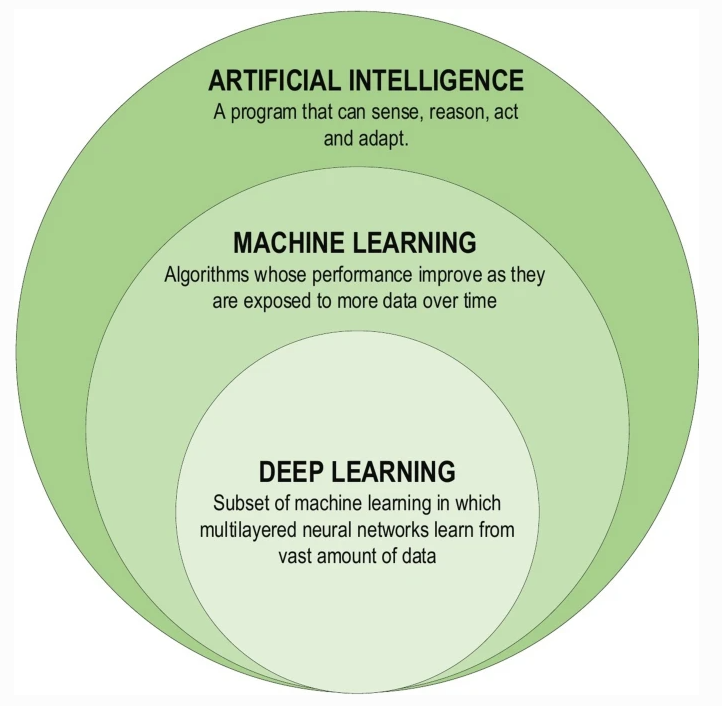
\includegraphics[scale=0.5]{images/ai family.png}\\
	\begin{footnotesize}
		\caption{AI family \cite{10}}
		\label{AI family}
	\end{footnotesize}
\end{figure}

\noindent In order to recognize patterns and connections that could escape the human eye, ML and DL algorithms, a subset of AI as shown in \ref{AI family} can analyze large and heterogeneous datasets, including genomes, medical imaging, and patient records. This not only speeds up the diagnosis procedure but also makes it possible to create individualized treatment programs that improve patient results. Additionally, AI-driven robotic devices are transforming surgical procedures by enabling minimally invasive interventions and increasing surgeons' abilities with increased precision and real-time data feedback.
Diverse industries have been transformed by AI and ML, giving professionals the tools they need to solve complex issues, improve decision-making, and spur creativity. The combination of AI and ML has increased production and efficiency while also creating new opportunities for social and scientific advancement. A future where AI and ML constructively contribute to human well-being and sustainable development must be encouraged as these technologies continue to advance. To do this, it is crucial to strike a balance between innovation and ethical considerations.

\begin{figure}[h]
\centering
	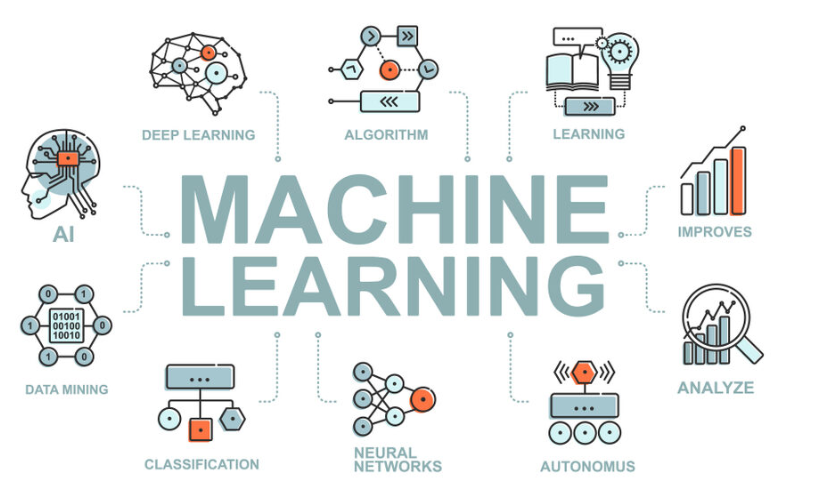
\includegraphics[scale=0.75]{images/machine learning.png}\\
	\begin{footnotesize}
		\caption{Machine Learning chart \cite{9}}
		\label{machine learning}
	\end{footnotesize}
\end{figure}

% \begin{figure}[h]
% \centering
% 	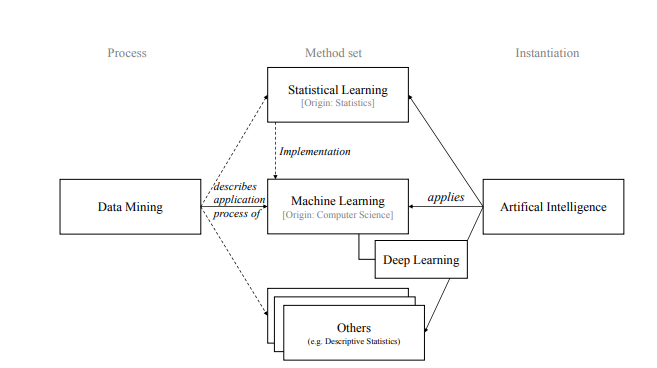
\includegraphics[scale=1.0]{images/terminology.png}\\
% 	\begin{footnotesize}
% 		\caption{Terminology \cite{19}}
% 		\label{de}
% 	\end{footnotesize}
% \end{figure}

\noindent The figure \ref{machine learning} is a comprehensive visualization of the intricate landscape surrounding machine learning (ML). It captures the wide range of ML types and the diagram outlines the steps of data mining, preprocessing, algorithm selection, model training, and analysis as it leads the observer through the complex process of machine learning. The figure serves as a focus point and expertly captures the core of machine learning, enabling a greater comprehension of its various forms, workings, and complex relationships.


\section{Importance of Data}
Data and datasets are of utmost importance in the field of machine learning, serving as the foundation for the entire structure of predictive modeling. As mentioned in \cite{44}, "What’s important to understand is that the value in data isn’t its rarity – the value is the potential and what we’re able to do with it".
Data provides an empirical foundation from which algorithms extract information, patterns, and correlations, allowing them to make predictions and educated conclusions. The correctness, completeness, and relevance of the data provided have a direct impact on how well machine learning models perform. A substantial dataset that has been carefully gathered and curated provides a thorough picture of the underlying phenomenon, enabling models to uncover complex correlations and nuanced details that might not be obvious otherwise.
A model becomes excessively fit to the training data, a phenomenon known as overfitting, and is unable to generalize to new, unobserved occurrences. The sheer volume of data also plays a crucial role in reducing the dangers of overfitting. Models may generalize beyond the training samples and effectively respond to unexpected circumstances when they are given large and diverse datasets, which provide the essential diversity of examples.

\noindent Additionally, the value of data extends beyond model development. The process of enhancing a dataset, perfecting feature engineering, and dealing with potential biases directly contributes to the ethical and responsible application of machine learning solutions. This promotes fairness and equity in decision-making by ensuring that the models lack reinforcing existing biases and inequities found in the data.
The value of data grows more and more obvious as machine learning spreads to more and more diversified industries, like healthcare, finance, agriculture, and others. It encourages inventions, leads to precise forecasts, and deepens our comprehension of complex processes. Therefore, the careful selection, growth, and improvement of datasets represent a crucial and continuing task, determining the development of machine learning and its revolutionary effects on society.





\section{Data analysis}
Data analysis is a critical step in research, business, and decision-making. It involves looking at and interpreting raw data to find important patterns, insights, and trends. It includes a broad range of methodologies, including fundamental descriptive statistics as well as more sophisticated approaches like data mining, machine learning, and statistical modeling. Data is prepared for analysis by being cleansed, arranged, and translated into a structured format during data analysis. Charts and graphs are popular visualization tools used to show facts visually and promote greater understanding.
The ultimate purpose of data analysis is to unearth relevant information that might support research hypotheses, assist decision-making, highlight opportunities or problems, and help organizations or enterprises develop strategies. Through data analysis, researchers and analysts may make sense of complicated datasets, identify patterns, and arrive at relevant conclusions that aid in the growth of numerous disciplines and support systems for making decisions using the best available evidence.

\begin{figure}[h]
\centering
	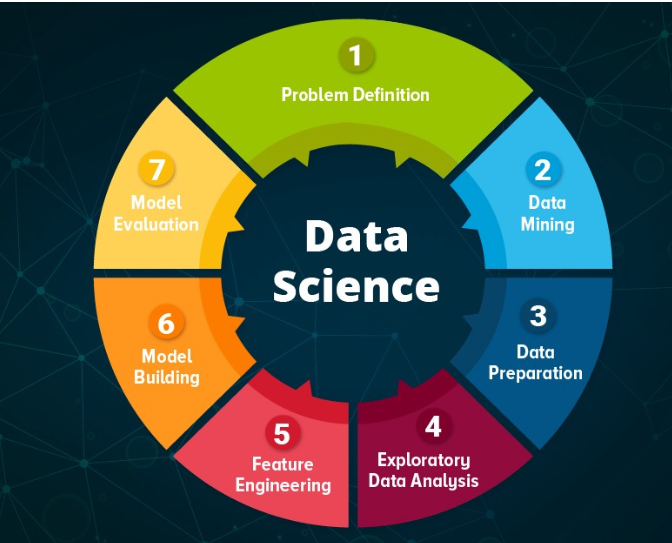
\includegraphics[scale=0.8]{images/data analysis.png}\\
	\begin{footnotesize}
		\caption{Data Analysis process chart\cite{12}}
		\label{data analysis}
	\end{footnotesize}
\end{figure}

\noindent Figure \ref{data analysis} provides a visual roadmap for the phases involved in the data science journey's successful implementation and captures its essence. It starts with the crucial problem definition phase, during which the fundamental goals are methodically outlined. Then, it leads us through the complex landscape of data science while laying out the sequential phases of data mining, a project designed to extract insightful knowledge from unstructured data. The illustration transitions between the important phases of data preparation and exploratory data analysis, illuminating their importance in enhancing and understanding the dataset's intricacies.
Further, the figure depicts the feature engineering refinement process, a creative undertaking that turns unstructured data into useful variables for modeling. The craft of developing models, where algorithms are carefully selected and adjusted to best suit the challenge at hand, is revealed as the process continues. The figure ends with the crucial phase of model evaluation, which is a thorough review of the model's performance in comparison to defined metrics. In essence, the figure serves as a clear and informative road map, condensing the complex nature of data science into an insightful narrative.


\bigskip
\bigskip
\bigskip
\bigskip
\bigskip
\bigskip
\bigskip
\bigskip
\bigskip
\bigskip
\bigskip
\bigskip
\bigskip
\bigskip
\bigskip
\bigskip
\bigskip
\bigskip
\bigskip
\bigskip
\bigskip
\section{Machine learning branches}
Machine learning can be divided into several subsets or branches, as shown in figure \ref{Machine Learning branches} each with its specific focus and applications. The main subsets of machine learning are:

% \begin{figure}[h]
% \centering
% 	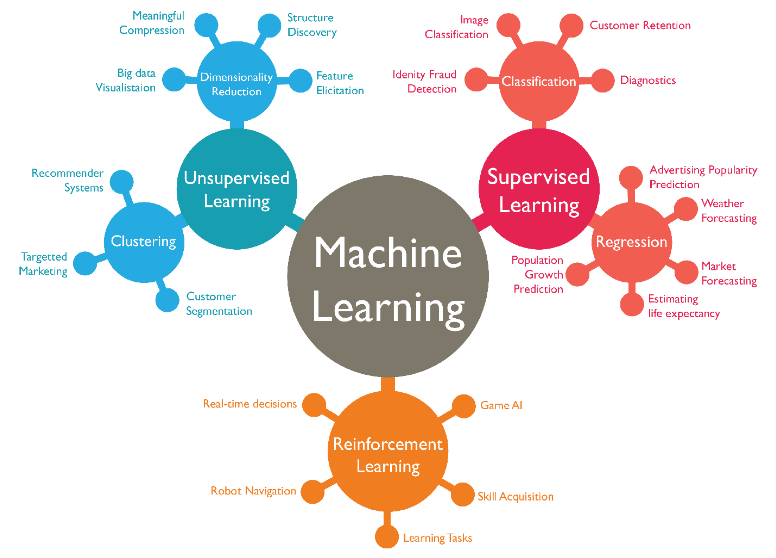
\includegraphics[scale=0.8]{images/ml branches.png}\\
% 	\begin{footnotesize}
% 		\caption{Machine Learning branches \cite{13}}
% 		\label{de}
% 	\end{footnotesize}
% \end{figure}


\begin{figure}[h]
\centering
	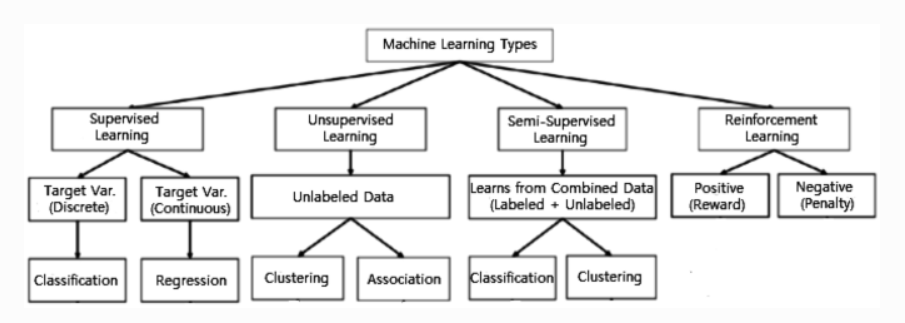
\includegraphics[scale=0.8]{images/ml techniques.png}\\
	\begin{footnotesize}
		\caption{Machine Learning branches \cite{22}}
		\label{Machine Learning branches}
	\end{footnotesize}
\end{figure}

\subsection{Supervised Learning}
The primary machine learning paradigm is supervised learning, where the algorithm is trained on a labeled dataset where each input data point has a corresponding target or label. A mapping from input features to output labels must be learned during the process of supervised learning for the algorithm to generate precise predictions on brand-new, untainted data. To reduce the difference between its predictions and the actual labels in the training data, the algorithm iteratively modifies its internal parameters, such as weights and biases, throughout the training phase. Usually, this optimization procedure uses backpropagation and gradient descent algorithms. Figure \ref{supervised learning} shows an overview of the supervised learning
approach. Two major categories of supervised learning are: Classification and 
Regression. 



\subsubsection{Classification}
Predicting the categorical class label of an input data point is the primary goal of the supervised learning problem of classification. In classification, the algorithm learns from a labeled dataset where each data point is assigned a class label. The goal is to create a model that can accurately classify fresh, untrained data elements into one of the predefined classes. Examples of common classification tasks include email spam detection (where emails are categorized as spam or not), picture recognition (assigning items in an image to specified classes), and medical diagnosis (categorizing patient conditions).

\subsubsection{Regression}
Regression is a form of supervised learning as well, but its output is a prediction of a continuous numeric value. Regression uses labeled data, where each data point has a matching numeric target value, to train the algorithm. The goal is to develop a model that can correctly forecast the desired value from fresh input data. Regression problems include evaluating crop production based on environmental parameters, projecting stock prices, and predicting housing prices based on features like size and location.

\begin{figure}[h]
\centering
	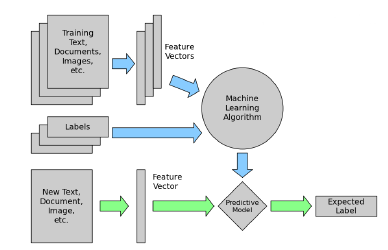
\includegraphics[scale=1.5]{images/supervised learning.png}\\
	\begin{footnotesize}
		\caption{supervised learning\cite{42}}
		\label{supervised learning}
	\end{footnotesize}
\end{figure}


\subsection{Unsupervised Learning}
Unsupervised learning is a branch of machine learning that deals with unlabeled data and seeks to identify underlying structures, relationships, or patterns without the use of explicit training data or predefined output labels. It is a more difficult and exploratory procedure than supervised learning because there is no "ground truth" to compare the algorithm's predictions to. Unsupervised learning algorithms instead concentrate on locating groups of related data points using methods like clustering or locating condensed versions of the data using dimensionality reduction. In contrast to dimensionality reduction approaches, which try to reduce the number of features while keeping important information, clustering algorithms combine data points based on their similarity. For data exploration, anomaly identification, and understanding the fundamental properties of the data, unsupervised learning is essential. It is essential for tasks where the true labels are unknown and where the algorithm needs to find hidden structures in order to extract meaningful information from the input. Figure \ref{unsupervised learning} shows an overview of the unsupervised learning
approach.

\subsubsection{Clustering}
Clustering is a fundamental technique in the field of unsupervised machine learning, aiming to uncover hidden patterns, similarities, and structures within data. It involves categorizing related data points into clusters or segments according to their inherent characteristics. Clustering's primary goal is to group data points so that they are more similar to one another than to those in other clusters. Through the detection of inherent correlations between data points, this approach can shed light on the dataset's underlying structure. Among its many uses are customer segmentation, image segmentation, anomaly detection, and recommendation systems, where it plays a crucial part in highlighting significant patterns in intricate and unstructured data, ultimately helping in making informed choices.

\begin{figure}[h]
\centering
	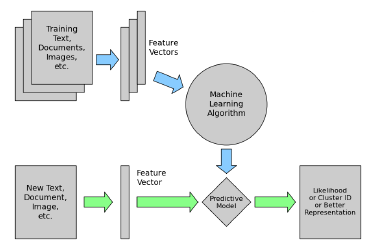
\includegraphics[scale=1.5]{images/unsupervised learning.png}\\
	\begin{footnotesize}
		\caption{unsupervised learning\cite{42}}
		\label{unsupervised learning}
	\end{footnotesize}
\end{figure}


\subsection{Semi-Supervised Learning}
Between supervised and unsupervised learning is semi-supervised learning. To train the model, it makes use of both labeled and unlabeled data. The algorithm's performance is improved because of the small amount of labeled data which assists it in learning from the unlabeled data. When gathering labeled data is expensive or time-consuming, semi-supervised learning is advantageous since it makes better use of the data that is already available.

\subsection{Reinforcement Learning}
A branch of machine learning called reinforcement learning is concerned with training agents ways to interact with the environment and gain knowledge from positive or negative feedback. Over time, the agent learns to operate in a way that maximizes cumulative rewards; this training depends on the concept of trial and error. This method is especially well suited for sequential decision-making problems seen in games, robotics, and autonomous systems.

\noindent Reinforcement Learning includes an environment and one or more agents. With the help of a chosen policy, these agents interact with the environment through acting. Following every interaction, the agent receives feedback (in the form of a reward) from the environment and modifies its state as required. Any intelligent entity, relevant to the issue is represented by an agent. The main goal of this approach is to maximize the total rewards accrued throughout an infinite number of exchanges. This strategy is encapsulated in the RL process as seen in Figure \ref{Reinforcement Learning}.\cite{43} 

\begin{figure}[h]
\centering
	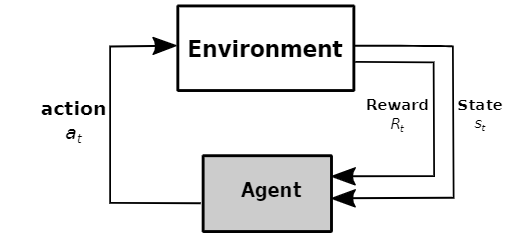
\includegraphics[scale=1.5]{images/Reinforcement Learning.png}\\
	\begin{footnotesize}
		\caption{Reinforcement Learning \cite{43}}
		\label{Reinforcement Learning}
	\end{footnotesize}
\end{figure}

\subsection{Deep Learning}
Deep learning is a specialized and sophisticated branch of machine learning that focuses on developing deep neural networks, which are multi-layered neural networks. In difficult problems like speech recognition, computer vision, and natural language processing, these networks have demonstrated remarkably good results. By gradually extracting more abstract information at each layer, the depth of the neural networks enables them to automatically develop hierarchical representations from unstructured data. The network's numerous variables are altered throughout the training phase, which is often carried out using large-scale datasets, in order to minimize the prediction error. Due to its ability for handling enormous volumes of data and comprehending intricate patterns, deep learning has revolutionized a number of industries and allowed for the creation of cutting-edge models with previously unheard-of capabilities and accuracy.

\subsubsection{Neural Network}
In the fields of artificial intelligence and Deep learning, a neural network is a fundamental idea that aims to replicate the extraordinary capabilities of the human brain. A neural network is made up of a number of nodes, or artificial neurons, stacked in layers and is inspired by the complex network of neurons and their connectivity in the brain. Each neuron receives input data, processes it by adding the inputs' weights together and adding a bias term, and then applies an activation function to the processed data to produce an output \cite{20}. By introducing non-linearity, the activation function enables neural networks to model complicated relationships and identify subtle patterns in the data.
An input layer, one or more hidden layers, and an output layer typically make up a neural network's architecture. As the input data spreads across the network, the hidden layers operate as intermediate representations, gradually extracting higher-level properties from the data. On the basis of the learnt representations from the hidden layers, the output layer generates the final prediction or decision. Ultimately, the goal is to minimize the cost function to ensure the correctness of fit for any given observation.\cite{21} Figure \ref{Neural Network Architecture} shows a simple schematic of a deep neural network.

\begin{figure}[h]
\centering
	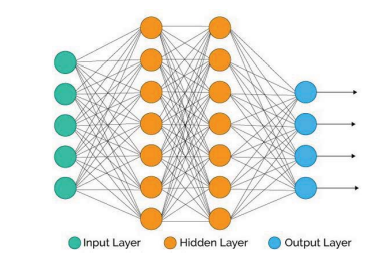
\includegraphics[scale=1.25]{images/neural network architecture.png}\\
	\begin{footnotesize}
		\caption{Neural Network Architecture\cite{11}}
		\label{Neural Network Architecture}
	\end{footnotesize}
\end{figure}

\noindent The ability of neural networks to learn complex and abstract representations from massive amounts of input is one of their primary benefits. They excel at tasks like picture identification, audio recognition, natural language processing, and more because of their ability to automatically find significant patterns in the data. Numerous sectors have been transformed by neural networks, which have helped advance applications for autonomous vehicles, healthcare diagnostics, agriculture, recommendation systems, and a plethora of other uses.
In order to advance artificial intelligence and address challenging real-world challenges, neural networks are expected to play an increasingly important role as they develop and change the machine learning environment.


\subsection{Transfer Learning}
Transfer learning is the process of using the skills developed when training a model for one job to enhance performance on a different but related task. Transfer learning involves refining a previously trained model on a fresh dataset in order to apply the learnt features to the fresh task. When the target dataset is small, transfer learning is helpful because it enables the use of information from a larger dataset or domain.
\bigskip
\bigskip

\noindent Each machine learning subset has unique abilities and tackles various issues. Depending on the unique properties of the data, the issue at hand, and the desired output, the right subset or combination of subsets should be chosen. The divisions between these subsets are becoming more flexible as machine learning develops, opening up new opportunities for study and applications in the area of artificial intelligence.




\section{Arabidopsis thaliana}
Thale cress or Arabidopsis thaliana is a small flowering plant that is a member of the Brassicaceae family. For a number of compelling reasons, it has become a popular model organism in plant biology research. The selection of Arabidopsis thaliana as the study plant in the context of this thesis report on biomass estimation using plant phenotype and machine learning models is well-justified, taking into account its numerous positive traits that support thorough and insightful research.

\noindent The exceptionally quick life cycle of Arabidopsis thaliana, which normally lasts six to eight weeks from seed germination to seed production, is one of the plant's major advantages. This quick life cycle makes it possible for researchers to run tests and see several generations develop in a short amount of time, which makes it easier to gather a wealth of data and quickens the speed of research. The research of various growth phases and responses to environmental changes is also made possible by the rapid return time, giving information on the dynamic features of plant growth and development.
Furthermore, there are several wild accessions of Arabidopsis thaliana that can be studied, demonstrating a high degree of genetic variety. The identification of important genetic elements controlling biomass accumulation and growth patterns is made possible by the genetic variety that allows researchers to examine a wide range of phenotypic features and reactions to various environmental situations. The diversity also improves the research's robustness and generalizability because conclusions drawn from several accessions are more likely to be relevant generally.
The modest size and simplicity of cultivation of Arabidopsis thaliana make it a useful plant for studies in greenhouses or other controlled environments. As shown in fig \ref{arabidopsis single} Its modest size makes data gathering and picture analysis much simpler, especially when using sophisticated phenotyping platforms like the ones discussed in this thesis report. The simplicity of culture also guarantees constant and repeatable experimental conditions, which minimizes potential confounding variables and improves the validity of research findings.

\begin{figure}[h]
\centering
	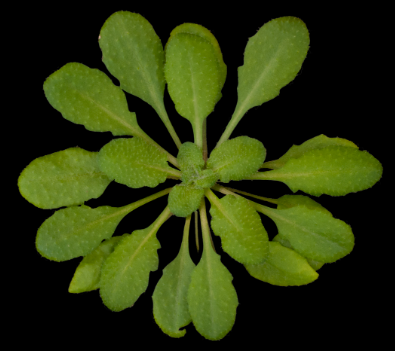
\includegraphics[scale=0.8]{images/arabidopsis single.png}\\
	\begin{footnotesize}
		\caption{Arabidopsis Thaliana \cite{14}}
		\label{arabidopsis single}
	\end{footnotesize}
\end{figure}

\noindent In conclusion, due to its short life cycle, small genome, genetic variety, genetic tractability, and ease of cultivation, Arabidopsis thaliana stands out as an essential model organism in this research project. Together, these beneficial characteristics offer researchers an effective set of tools that they can use to investigate the nuances of plant phenotype, understand the nuanced mechanisms governing biomass estimation, and investigate the exciting potential of machine learning models in the fields of agriculture and plant biology. This thesis report uses the study of the plant Arabidopsis thaliana to advance biomass estimation procedures and deepen our comprehension of the dynamics of plant growth in response to environmental factors. Figure \ref{Arabidopsis Thaliana from the experiment} represents a top view image from the experiment.

\begin{figure}[h]
\centering
	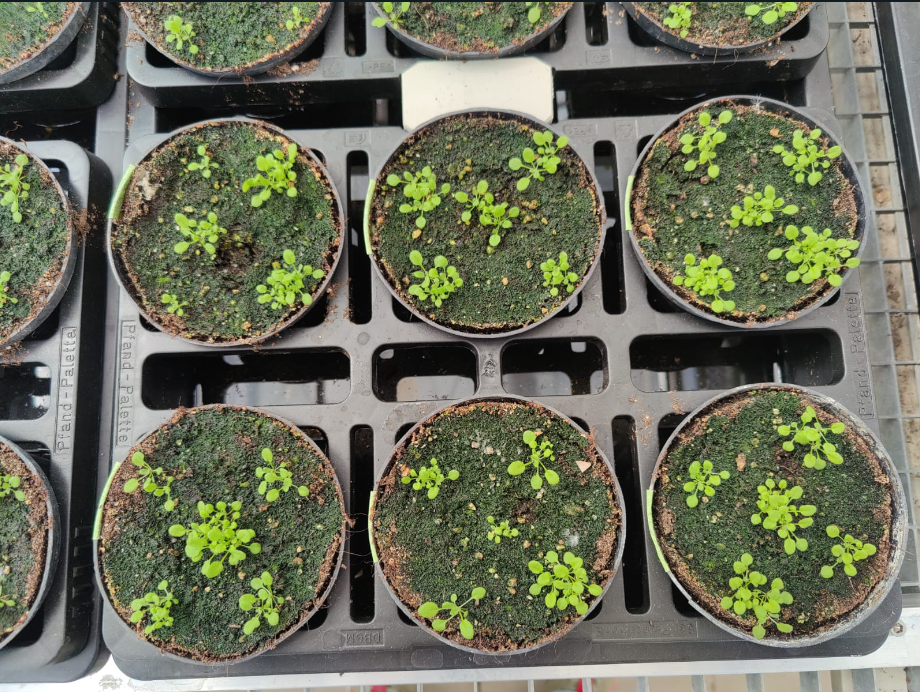
\includegraphics[scale=1.0]{images/Arabidopsis.png}\\
	\begin{footnotesize}
		\caption{Arabidopsis Thaliana from the experiment}
		\label{Arabidopsis Thaliana from the experiment}
	\end{footnotesize}
\end{figure}


\section{Plant phenotype}
The term "plant phenotype" describes the observable physical and physiological characteristics of a plant that are the outcome of how its genotype interacts with its environment. Plant height, leaf form, flower color, the architecture of the root system, and reactions to biotic and abiotic stressors are only a few examples of the qualities that these attributes cover. The complex interplay between a plant's DNA and the environmental conditions it experiences throughout its life cycle result in its phenotypic.
It is essential in determining the ability of plants to respond to various environmental cues, tolerate fluctuations, and engage in ecosystem interactions. In order to improve agricultural productivity, resilience, and nutritional value, breeders must be able to choose and create plants with desirable qualities, which requires a thorough understanding of plant phenotypes. Studying plant phenotypes also aids in understanding how plants react to disease, climate change, and other ecological factors, providing insights into ecosystem dynamics and biodiversity conservation. A deeper knowledge of plant phenotypes has been made possible by improvements in high-throughput phenotyping tools and imaging methods, advancing plant biology and agriculture.


\section{Image processing}
Within the broader field of computer vision, image processing is a specialized and comprehensive science devoted to modifying, analyzing, and enhancing digital images in order to gain insightful knowledge, enhance visual quality, and facilitate the extraction of useful information. Image processing is essential to many applications across a wide range of sectors as the world grows more visually oriented.
Images are represented as two-dimensional arrays of pixels in digital image processing, where each pixel carries information about the color or grayscale intensity of an image. Spatial domain processing and frequency domain processing are the two basic categories under which image processing techniques can be divided. Spatial domain processing entails carrying out operations directly on the image's pixel values. Image filtering, which blurs or sharpens the image, edge detection, which draws attention to the borders between various sections, and image enhancement, which seeks to enhance visual quality by modifying brightness, contrast, and color balance, are common procedures.

\noindent The rapid development of computing power, which has resulted in the creation of more intricate and sophisticated algorithms, is largely responsible for the continuing advancement of image processing. Machine learning's branch of deep learning, which enables cutting-edge approaches to image recognition, segmentation, and synthesis, has also made a significant contribution to image processing.
The way we view and interact with the visual environment has been completely transformed by the important field of image processing. Our daily lives have been made better by its numerous uses across numerous industries, which have also aided in scientific developments, medicinal advances, and technology advances. The future will surely be shaped by image processing as it develops, pushing the frontiers of what is feasible in the field of computer vision and beyond. 

\begin{figure}[h]
\centering
	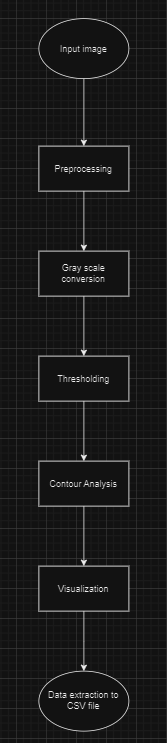
\includegraphics[scale=1.0]{images/image processing steps.png}\\
	\begin{footnotesize}
		\caption{Image processing steps}
		\label{Image processing steps}
	\end{footnotesize}
\end{figure}

\noindent The flowchart in Figure \ref{Image processing steps} outlines a systematic image processing workflow for analyzing images. The process begins with the input of the image, which is then subjected to necessary preprocessing measures to improve its quality and suitability for analysis. which includes Noise reduction, and scaling of the images. Subsequently, the image is converted to grayscale, simplifying its structure and preparing it for further analysis.
The grayscale image then moves on to the thresholding phase, where it undergoes a binary image transformation that effectively separates the foreground and background depending on intensity levels. Then, using specialized algorithms, the contour analysis of this binary image is performed in order to identify discrete object boundaries. These lines define the shapes of the objects seen in the image.
The flowchart then continues by superimposing the identified outlines onto the original image to see the outcomes. The segmentation and contour analysis procedures' accuracy is checked as part of this visualization step. Additionally, the extracted data is based on the identified contours.
The extracted data is organized and saved to a CSV (Comma-Separated Values) file, and it includes the required properties of the image. This organized output makes it easier to do additional analysis. Overall, this flowchart offers a systematic method for converting unprocessed image input into informative and quantifiable data, enabling thorough image analysis and interpretation.


\subsection{Computer vision}
% A robust and popular open-source computer vision and image processing library is OpenCV (Open Source Computer Vision Library). It offers a large selection of functions and algorithms for image and video analysis, object detection, feature extraction, machine learning, and more. OpenCV was originally developed by Intel and is now maintained by the community. With support for numerous programming languages like C++, Python, Java, and MATLAB, OpenCV is made to be effective, cross-platform, and simple to use. In a variety of fields, including robotics, augmented reality, autonomous cars, and medical imaging, its adaptability has made it a popular choice for researchers, developers, and students. OpenCV is a crucial tool for creating computer vision applications that has considerably advanced the fields of computer vision and image processing, whether it is for image filtering, edge detection, facial recognition, or video tracking.

The fields of computer vision and image processing are closely related and collaborate to provide machines with the ability to comprehend and interpret the visual environment. Image processing, which uses a variety of methods to enhance and preprocess digital images to make them more acceptable for further analysis, serves as the foundation for computer vision. To enhance image quality, reduce noise, and isolate regions of interest, techniques including filtering, denoising, and image segmentation are essential. Following the preprocessing of the images, computer vision algorithms assume control and use the data obtained from image processing to carry out complex tasks like item recognition, scene interpretation, and even human position estimates.
Thanks to the synergy between computer vision and image processing, machines can identify their surroundings, recognize objects and patterns, and make intelligent decisions based on visual data. The development of autonomous vehicles, medical diagnostics, surveillance systems, augmented reality applications, and other fields have all been made possible by this potent combination, which has changed many different industries. We can anticipate far more noteworthy advances as the fields evolve and advance, which will improve our comprehension of the visual environment and spur innovation in a variety of fields. Figure \ref{Computer Vision} provides a simple overview of Computer Vision application.

\begin{figure}[h]
\centering
	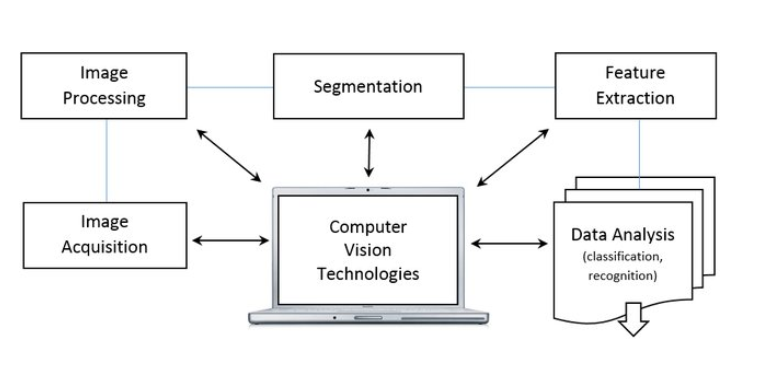
\includegraphics[scale=1.0]{images/image processing.png}\\
	\begin{footnotesize}
		\caption{Computer Vision \cite{15}}
		\label{Computer Vision}
	\end{footnotesize}
\end{figure}





\subsection{Thresholding}
A fundamental method in image processing called thresholding is used to convert grayscale or color images into binary images. To divide an image's pixel intensities into foreground and background classes, a threshold value must be established. Pixels assigned to the foreground class and often represented as white have intensities higher than the threshold, whereas pixels assigned to the background class and typically represented as black have intensities lower than or equal to the threshold. Thresholding is very helpful for separating objects or areas of interest from the background in an image, which makes activities like feature extraction and additional analysis easier. The selection of the threshold value is crucial and is based on the unique qualities of the image as well as the intended segmentation result.
To fit varied image types and applications, a variety of thresholding approaches, including global thresholding, adaptive thresholding, and Otsu's thresholding, are available. Thresholding is frequently used in tasks like object detection, character recognition, and image preprocessing for computer vision and machine learning applications. Thresholding properly implemented can considerably increase image segmentation accuracy.


\subsection{Contours}
The boundaries of objects or regions with comparable pixel intensity or color are represented by continuous curves called contours in image processing. They are essential for object recognition and form analysis. Contours are made up of connected points that outline the forms in an image and are detected by edge detection or thresholding. In order to characterize and categorize objects, contour information can be used to extract useful properties like area, perimeter, and orientation. The ability for machines to comprehend and interact with the visual environment based on shape-based information is made possible by contours, which are vital in computer vision tasks including object detection, image segmentation, and gesture recognition.



\section{Important terms and concepts}
\subsection{Scikit-learn (sklearn)}
Popular machine learning library Scikit-learn offers a full range of tools for various machine learning tasks, including as classification, regression, clustering, dimensionality reduction, and more. It is meant to be user-friendly and effective and is built on top of other scientific Python libraries like NumPy and SciPy. Both beginners and seasoned machine learning practitioners can use Scikit-learn because of its consistent API and variety of algorithms. It offers modules for model training, evaluation, hyperparameter adjustment, feature selection, and data preprocessing. Furthermore, Scikit-learn easily interfaces with other Python tools, allowing programmers to quickly create end-to-end machine learning pipelines.

\subsection{Pandas}
Python has a robust data analysis and manipulation module called Pandas. It provides simple data structures, principally the DataFrame, that enable users to efficiently work with labeled and structured data. Users can execute necessary data cleaning, transformation, and manipulation activities with Pandas and import data from a variety of file formats, including CSV, Excel, and SQL databases. It offers features for data wrangling and preparation, including filtering, sorting, grouping, aggregating, and merging. Additionally, Pandas is made to integrate easily with other NumPy and Matplotlib-compatible scientific Python tools, allowing users to swiftly complete challenging data analysis and visualization jobs.

\subsection{R-squared value (coefficient of determination)}
A statistical metric used to assess the goodness of fit of a regression model is the R-squared value, sometimes referred to as the coefficient of determination. It measures the percentage of the variance in the dependent variable's output that can be accounted for by the model's independent variables' inputs \cite{23}. The R-squared value ranges from 0 to 1, where a value of 0 means that the model does not explain any variance in the dependent variable, and a value of 1 means that the model perfectly fits the data and fully accounts for all variance. Higher R-squared values, in general, show that the model fits the data better and that the predictions of the model closely match the actual data points. To prevent overfitting and ensure the model's validity for making correct predictions on fresh, unforeseen data, R-squared must be interpreted in conjunction with other evaluation metrics and domain expertise.

The coefficient of determination, \( R^2 \), is calculated using the formula \cite{24}:

\[
R^2 = 1 - \frac{SS_{\text{res}}}{SS_{\text{tot}}}
\]

where:
\begin{align*}
R^2 & \text{ is the coefficient of determination,} \\
SS_{\text{res}} & \text{ is the sum of squares of the residuals (SSE), representing unexplained variability, and} \\
SS_{\text{tot}} & \text{ is the total sum of squares, representing the total variability in the data.}
\end{align*}


\subsection{Mean squared error (MSE)}
The average squared difference between projected values and actual values in a regression or estimation problem is measured by the mean squared error (MSE), a commonly used statistical metric. It is a crucial performance indicator for the assessment of the accuracy of a prediction model \cite{25}. The difference between each predicted value and its associated actual value is squared in order to calculate MSE, which is then calculated as the average of these squared disparities. The outcome value offers an indicator of how well the model's predictions reflect the actual values. A lower MSE suggests a more accurate and precise model because it shows that the model's predictions are more in line with the actual values. 
Overall, the MSE is a useful tool for evaluating the effectiveness of regression models, assisting in the choice of models, and directing efforts to improve models.

The Mean Squared Error (MSE) is calculated using the formula \cite{26}:

\[
\text{MSE} = \frac{1}{n} \sum_{i=1}^{n} (y_i - \hat{y}_i)^2
\]

where:
\begin{align*}
\text{MSE} & \text{ is the Mean Squared Error,} \\
n & \text{ is the number of data points,} \\
y_i & \text{ is the actual (observed) value of the dependent variable for the } i\text{th data point, and} \\
\hat{y}_i & \text{ is the predicted (estimated) value of the dependent variable for the } i\text{th data point.}
\end{align*}


\subsection{Mean Absolute Error (MAE)}
A key metric for evaluating the precision of predictive models, especially in the context of regression analysis, is mean absolute error (MAE). The average size of the differences between the expected and actual values is evaluated. In particular, MAE computes the average of these absolute differences between each predicted price and its corresponding actual value.
The basic description of MAE is that it indicates the correctness of the model which means, the lower the MAE value, the closer the predicted values are to the actual values. It is an effective tool to evaluate model performance since it is resistant to outliers and gives an accurate picture of the magnitude of errors without reverence to their direction. In essence, MAE is a useful tool for evaluating the accuracy and dependability of regression models since it offers a brief indicator of how well a model's predictions reflect the actual observed values.

The Mean Absolute Error (MAE) is calculated as \cite{41}:

\[
MAE = \frac{1}{n} \sum_{i=1}^{n} |x_i - \hat{x}_i|
\]

where:
\begin{align*}
n & : \text{Number of data points} \\
x_i & : \text{Actual value of the } i\text{-th data point} \\
\hat{x}_i & : \text{Predicted value of the } i\text{-th data point}
\end{align*}



\subsection{Hyperparameter tuning}
Determining the ideal settings for hyperparameters, which are parameters set prior to the model's training that influence its performance and behavior, is a crucial step in the machine learning process of tuning hyperparameters. 
As can be seen in the above figure \ref{Hyperparameter tuning model}, Hyperparameters are determined by the developer or data scientist before training and have a substantial impact on the model's generalization and effectiveness, contrast with model parameters, which are learned from the training data (such as weights in a neural network). Learning rates, regularization strengths, the number of hidden layers in a neural network, and the number of trees in a random forest are examples of common hyperparameters. In order to determine the configuration that yields the highest performance on a validation set, hyperparameter tuning systematically examines various combinations of hyperparameter values.
This often involves the use of methods like grid search, random search, and Bayesian optimization. As a result, more robust and trustworthy machine learning models may be produced. Appropriate hyperparameter tuning can greatly increase the model's accuracy and minimize problems like overfitting or underfitting.

\begin{figure}[h]
\centering
	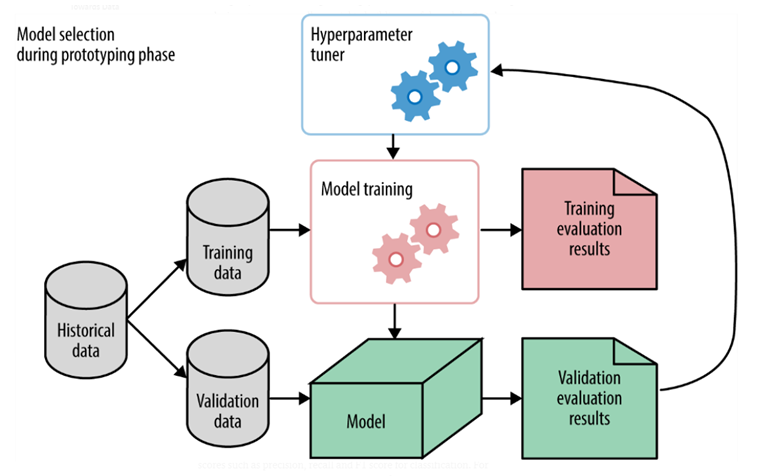
\includegraphics[scale=1.0]{images/hyperparameter tuning.png}\\
	\begin{footnotesize}
		\caption{Hyperparameter tuning model \cite{16}}
		\label{Hyperparameter tuning model}
	\end{footnotesize}
\end{figure}



\subsection{Cross-validation}
A reliable and popular method in machine learning for evaluating a model's performance and reducing the danger of overfitting is cross-validation. It entails partitioning the dataset into numerous folds or subsets, referred known as "k-folds." The model is tested on the remaining fold after being trained on folds k-1. Each fold is used as the validation set exactly once during the course of the next k iterations of this operation. The average of the evaluation outcomes from each of the k folds serves as the final performance statistic. Since the model may be evaluated on other data points that it hasn't encountered during training, cross-validation yields a more accurate estimate of the model's generalization capabilities.
As the model is assessed on various data partitions, decreasing reliance on a single train-test split, it also helps in spotting potential overfitting concerns. K-fold cross-validation, stratified k-fold cross-validation (used for imbalanced datasets), and leave-one-out cross-validation (used when the dataset is small) are three commonly used cross-validation techniques. Cross-validation is an essential phase in the development of a model since it directs hyperparameter tuning, influences model choice, and aids in the creation of more reliable and reliable machine learning models.

\subsection{Overfitting and underfitting}
The performance and generalizability of a model are both impacted by two prominent machine learning problems overfitting and underfitting as shown in Figure \ref{ofuf}.

\noindent The two key concepts that are closely related to the issues of overfitting and underfitting are bias and variance.

\bigskip
\noindent\textbf{Bias:} Bias is the error that results from using a model to approximate a complicated real-world problem. It symbolizes the model's tendency to consistently forecast target values incorrectly or correctly. High bias happens in the setting of underfitting when the model is too simple to discern the underlying trends in the data. As a result, regardless of the training data, the model constantly makes incorrect predictions. Increasing the complexity or capacity of the model is frequently necessary to address significant bias.

\bigskip
\noindent\textbf{Variance:} Contrarily, variation illustrates how sensitive a model is to subtle changes or background noise in training data. High variance suggests that the model is very sensitive to the training set and that it is more likely to capture noise than the true underlying patterns. This is frequently related to overfitting, a situation in which the model fits the training data too closely and struggles to generalize to new, untried data.




\begin{figure}[h]
\centering
	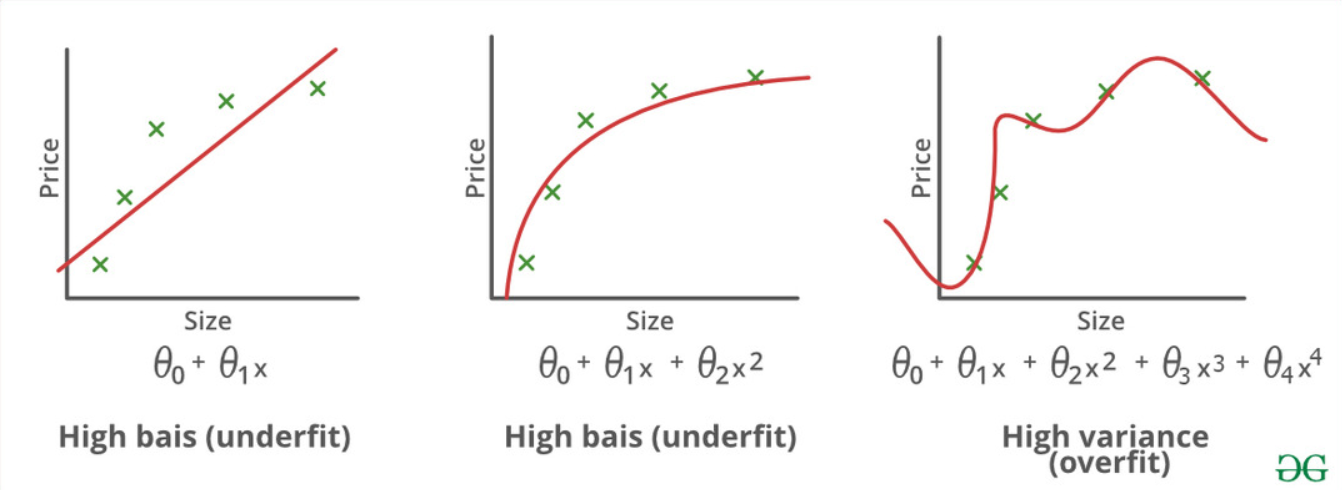
\includegraphics[scale=0.55]{images/ofuf.png}\\
	\begin{footnotesize}
		\caption{Bias and Variance Trade-Off  \cite{43}}
		\label{ofuf}
	\end{footnotesize}
\end{figure}


\bigskip
\noindent When a model becomes overly complicated, it learns to recognize noise or random oscillations in the training data rather than the underlying patterns, which is known as overfitting. As a result, although the model excels on the training data, it is unable to generalize to brand-new, untried data. Because the model has grown too dependent on the training data and is unable to manage variances in various datasets, overfitting can result in subpar performance on real-world tasks.
Underfitting, on the other hand, occurs when a model is simple and fails to recognize the underlying patterns in the training data. Due to its inability to recognize the true relationships between the input features and the target variable, an underfit model performs badly on both the training data and the fresh data. Underfitting frequently means that the model is unable to adequately capture the complexity of the data.
Techniques like regularization, early halting, and model complexity reduction can be utilized to alleviate overfitting. These techniques penalize excessively complicated models and stop them from remembering noise. More complicated models, feature engineering, or more data can allow the model to better catch significant trends in order to counteract underfitting.

\noindent Building reliable and accurate machine learning models that can perform well on new, untested data requires striking a balance between overfitting and underfitting. It is crucial to regularly evaluate the model using methods like cross-validation to make sure it generalizes well and can handle real-world scenarios successfully.



\chapter{Methodology}
A systematic strategy is used in the proposed methodology for the thesis report on biomass estimation utilizing plant phenotypic and machine learning models to address the challenges with conducting accurate and non-destructive biomass assessment. A comprehensive and representative dataset of plant phenotypic data, including characteristics like leaf area, and leaf length, will first be gathered. To guarantee the data's quality, it will go through an extensive preprocessing process that takes into account things like image resolution inconsistencies, shadows, and imaging artifacts. The preprocessed data will next be used to extract relevant and discriminative features using the appropriate methods. These features will capture crucial details pertaining to biomass estimation. Then, four effective machine learning algorithms will be chosen for the task: Random Forest (RF), Support Vector Machine (SVM), Multilayer Perceptron (MLP), and k-Nearest Neighbors (k-NN). Cross-validation techniques will be used to train the models on the preprocessed data, ensuring generalizability and reducing the risk of overfitting. To gauge their precision and robustness, their performance will be examined using appropriate metrics like mean squared error and accuracy.

\noindent To comprehend the connections between the phenotypic characteristics and biomass estimation offered by the models, interpretability approaches will also be used. The best machine learning (ML) model(s) will be chosen through comparative analysis based on performance, interpretability, and applicability to biomass estimation. In the end, a script will be created to automate the estimation of biomass, allowing for non-destructive, scalable, and effective evaluation. By employing this methodology, the thesis seeks to advance biomass estimation and offer fresh perspectives, with possible applications in forestry, agriculture, and environmental studies.

\section{Data Collection}
At the University of Cologne, about 540 Arabidopsis thaliana plants were grown within the constraints of a perfectly regulated glasshouse environment as part of a carefully planned data collection operation. As shown in Figure \ref{Plant arrangement in glasshouse for data collection}, the botanical subjects were meticulously spread throughout 192 different pots, which were then grouped into 16 trays, to ensure an orderly and comprehensible pattern. These trays can fit 12 pots on each, enabling a planned and organized growth arrangement.
Each plant had a thorough program of diligent maintenance over a five-week period that was closely observed, including regular measurements and exact weight assessments. A tremendously varied variety of samples from the Arabidopsis thaliana species were obtained thanks to this practical and methodical technique. This collection accurately captured the innate variety of this plant species by encompassing a wide range of shapes, sizes, and weights.

\begin{figure}[h]
\centering
	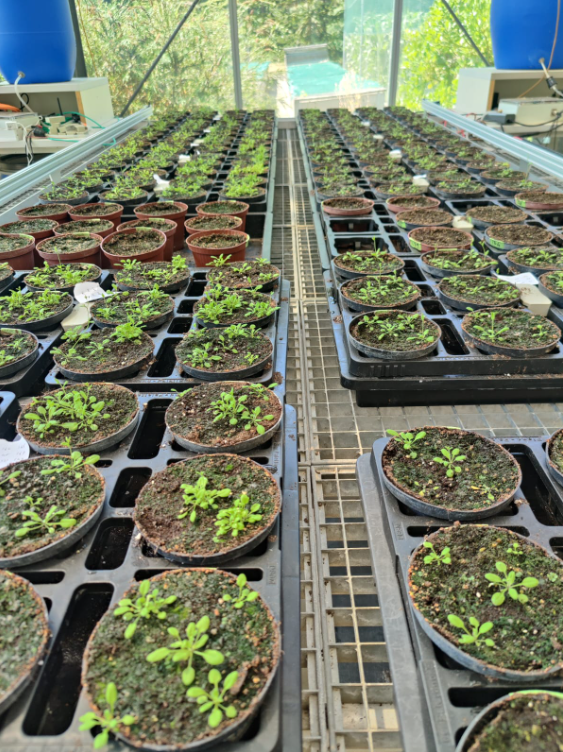
\includegraphics[scale=1.0]{images/data collection.png}\\
	\begin{footnotesize}
		\caption{Plant arrangement in glasshouse for data collection}
		\label{Plant arrangement in glasshouse for data collection}
	\end{footnotesize}
\end{figure}

\noindent The precise measurement and documentation of each plant's biomass, a vital feature that enhances the depth and richness of the dataset, was central to this attempt. These carefully collected biomass measurements were methodically incorporated into the dataset, enhancing its utility as a reliable training and testing resource for the machine learning models. 
The insightful glasshouse experiments, which produced a plethora of priceless data, were crucial to this data collection effort. A thorough and reliable dataset was created by seamlessly fusing the results of these studies with the earlier-captured photos. This dataset, which was carefully created, acts as the foundation for the training of complex machine learning models. These models, which have been carefully developed, have the potential to estimate biomass within the Arabidopsis thaliana species with accuracy.



\subsection{Plant material}
The seeds underwent a period of preservation at a controlled temperature of 4 degrees Celsius before they were sown into the pots. This step was performed to ensure the preservation of their vitality and wellbeing. A consistent and trustworthy dataset designated for biomass estimation purposes was established as a result of the uniform germination and subsequent growth of the plants in this controlled storage environment. In addition to making it easier to obtain this dataset, the use of Arabidopsis thaliana plants and a precise culture routine also made it possible for the careful investigation of numerous phenotypic features.
This coordinated strategy, which carefully monitored the growth circumstances and took advantage of Arabidopsis thaliana's special qualities, helped to increase the accuracy and efficacy of the suggested methodology for estimating biomass. This strategy has the promise of revealing deeper insights into the complex world of biomass estimation when combined with modern plant phenotyping methods and machine learning models.



\subsection{Image acquisition}
A Sandberg USB Webcam with a resolution of 1080p and a 2 megapixel sensor was used to take pictures inside the glasshouse. It was specifically created to give exacting image clarity. The webcam's USB interface makes it simple to use with a wide range of devices that have USB ports, including laptops, desktop PCs, and tablets. Because of its inherent adaptability, it is a sensible option for a variety of circumstances. The final images are meticulously recorded and saved in the widely used JPG/JPEG format. Figure \ref{Images captured from the camera} shows examples of the images acquired.

\begin{figure}[h]
\centering
	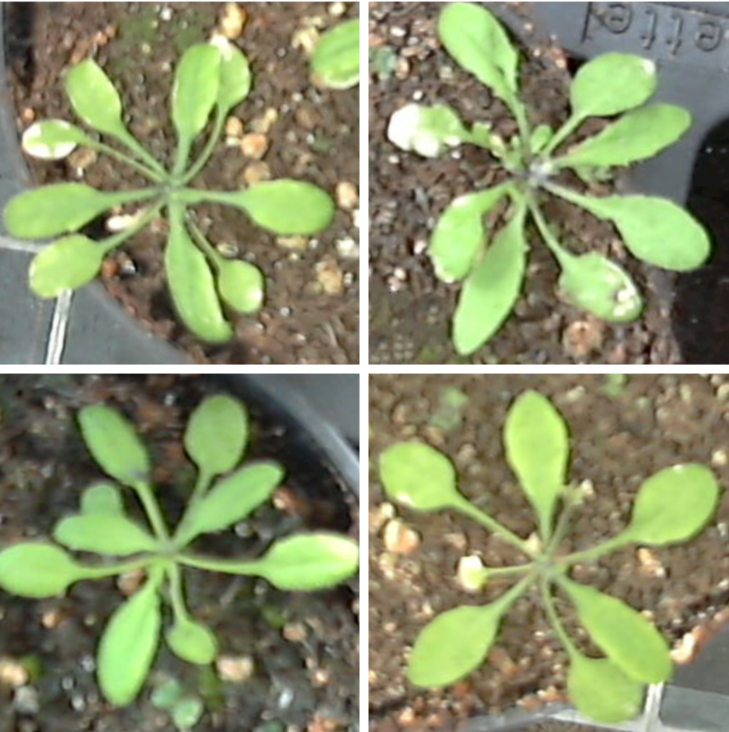
\includegraphics[scale=1.0]{images/images from camera.png}\\
	\begin{footnotesize}
		\caption{Images captured from the camera}
		\label{Images captured from the camera}
	\end{footnotesize}
\end{figure}


\section{Preprocessing and  Feature Extraction}
The main objective of this study is to construct biomass estimation models using a simplified method that considers two essential traits which are, the number of leaves and the leaf area of the plant. With these two characteristics acting as the primary input elements, the goal is to forecast the plant's biomass, which serves as the output variable. A wide and representative collection of plant images as well as measurements of the quantity, size, and fresh weight of the leaves are gathered in the first step of the procedure. The dataset includes a wide range of growth phases to guarantee the models' capacity to generalize.

\begin{figure}[h]
\centering
	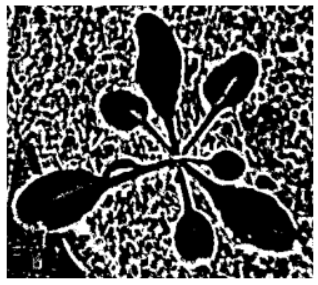
\includegraphics[scale=1.5]{images/Thresholding.png}\\
	\begin{footnotesize}
		\caption{Thresholding}
		\label{Thresholding}
	\end{footnotesize}
\end{figure}


% \noindent Upon gathering the dataset, preprocessing techniques are used to efficiently deal with noise, inconsistencies, and image artifacts. The study will then concentrate on feature extraction methods to extract useful information from the plant images, with a focus on pertinent features related to leaf area and leaf count in particular. While contour analysis is used in this context, various other methods can also be taken into consideration for the same task, including picture segmentation, shape descriptors, and texture analysis. The main objective is to determine the best technique for biomass estimation that accurately captures the important traits of the plants.


\noindent The images that make up the data set serve as the starting point from which extracts essential botanical attributes, namely the leaf area and count. In order to achieve this, sophisticated computer vision techniques are used, with contours and thresholding emerging as the preferred tools. Due to their ability at extracting and defining the intricate shapes of leaves from their often complex and varied surrounds, these techniques were strategically adopted. As shown in Figure \ref{Thresholding}, by efficiently separating the leaves from the backdrop via thresholding, the image is divided into binary sections based on pixel intensity. Then, using the contours approach, the edges of these divided leaves are carefully traced, enabling precise measurement of their dimensions.
Each image in the collection is subjected to this complex process, which results in a complete and reliable set of values for leaf area and count. These measures, which represent essential morphological traits, are carefully collated and structured within a CSV file.

\noindent The weight measurements are combined with the CSV file, which was obtained in the earlier processes, and then fed into the created models. This complex process is a key component of the methodology because it skillfully combines the organizational prowess of data processing and storage with the effectiveness of computer vision techniques. In the end, this combination produces and painstakingly perfects a model that excels in precision and flexibility and successfully predicts biomass estimation within the domain of Arabidopsis thaliana. 

\begin{figure}[h]
\centering
	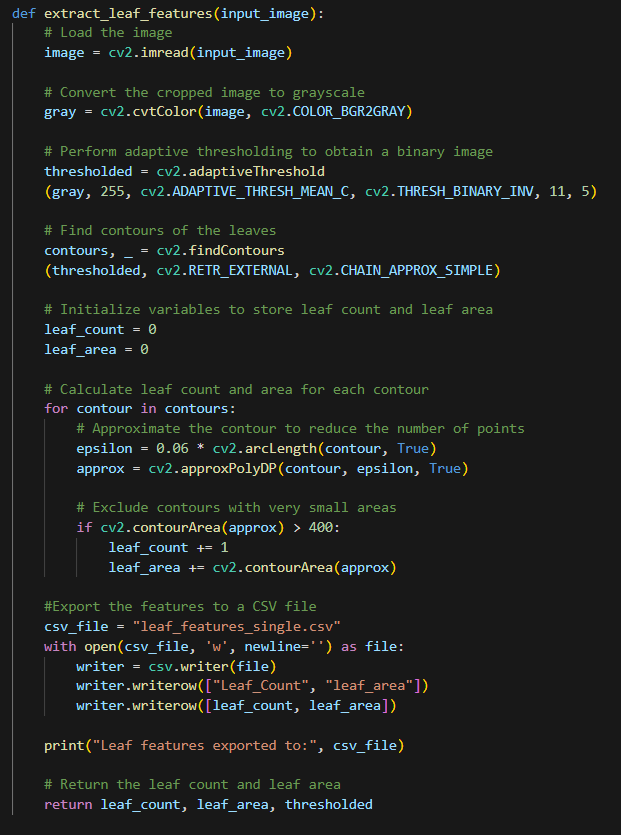
\includegraphics[scale=0.95]{images/extract features.png}\\
	\begin{footnotesize}
		\caption{Feature extraction script}
		\label{Feature extraction script}
	\end{footnotesize}
\end{figure}

\noindent A number of crucial image processing operations are carried out by the Python function extract\_leaf\_features in order to completely investigate plant leaves as shown in figure \ref{Feature extraction script}. The function subsequently continues on converting the input image into grayscale. This grayscale conversion is crucial because it reduces the image to its luminance values, which makes the subsequent computational tasks simpler.
The next stage uses adaptive thresholding, a method that effectively differentiates the plant leaves from the background. A binary image is produced as a result, with the leaves being emphasized and the backdrop being muted. Adaptive thresholding uses a particular algorithm called cv2.adaptiveThreshold to achieve optimal thresholding through localized modifications.
The script uses the findContours() method to accurately identify each individual leaf. These contours effectively serve as the leaf's borders and allow for accurate quantification and analysis. Notably, the options cv2.RETR\_EXTERNAL and cv2.CHAIN\_APPROX\_SIMPLE are used to make sure that just the outer leaf contours are collected and that the contour points are saved in an easy-to-use manner.
The function then continues on to the phase of leaf-by-leaf analysis. Each detected contour is iterated over, its area is calculated while approximating its shape to reduce computing complexity. The analysis is made more accurate by omitting minor or insignificant regions by discarding contours with negligible areas.
The function also averages the values for cumulative leaf area and leaf count. These computed parameters are then saved in a structured CSV file, making it simple to access them for additional research and visualization.

\noindent The function also averages the values for cumulative leaf area and leaf count. These computed parameters are then saved in a structured CSV file, making it simple to access them for additional research and visualization.
The computed leaf count and the total leaf area are the function's two important outputs. This comprehensive examination, contained in the returned values, provides a thorough understanding of the traits of the plant leaves in the input image. In conclusion, the extract\_leaf\_features function simplifies the analysis of plant leaves by allowing precise and effective extraction of critical data from images for innovative research and understanding of plant biology and agriculture.





\section{Model Development and Training}
This section explains the development of prediction models for biomass estimation. For this, the Random Forest (RF), Support Vector Machine (SVM), Multi-Layer Perceptron (MLP), and k-Nearest Neighbors (kNN) models have been used. Due to their distinct benefits and qualities, these models have been carefully considered. Complex relationships in data are easily handled by Random Forest, which is renowned for its ensemble nature. Nonlinear classification challenges are a strong suit for the robust Support Vector Machine. The Multi-Layer Perceptron, a crucial component of neural network topologies, is excellent at detecting complex patterns and hierarchies. Classification and regression tasks are successfully handled by k-Nearest Neighbors, which relies on proximity-based concepts.
This intentional combination of models guarantees a thorough investigation of predictive abilities, enabling a more informed choice of the best model for biomass estimation.


\subsection{Random Forest}
Random Forest (RF) regression is a machine learning algorithm used for biomass estimation based on the attributes of the number of leaves and leaf area extracted from plant images. RF regression is a powerful and versatile ensemble learning technique that combines multiple decision trees to create a robust predictive model.
The RF algorithm builds several decision trees, each of which is trained on a different subset of the dataset. These decision trees are created using a random subset of the training samples and a random selection of characteristics. Based on the input attributes (number of leaves and leaf area), each tree independently predicts the output variable (in this case, fresh weight) during the training phase. By averaging or collecting the majority vote of all the forest's trees' estimates, the final prediction is obtained.
The ability of RF regression to handle intricate interactions between input characteristics and the output variable is one of its primary advantages. The algorithm's ability to capture non-linear and interaction effects is particularly helpful in situations where there may not be a linear relationship between the number of leaves, leaf area, and fresh weight. RF regression can reveal complex connections and patterns that may not be seen using conventional statistical techniques. Figure \ref{Diagrammatic representation of a random forest} provides a systematic representation of a random forest model, which is composed of multiple decision trees

\begin{figure}[h]
\centering
	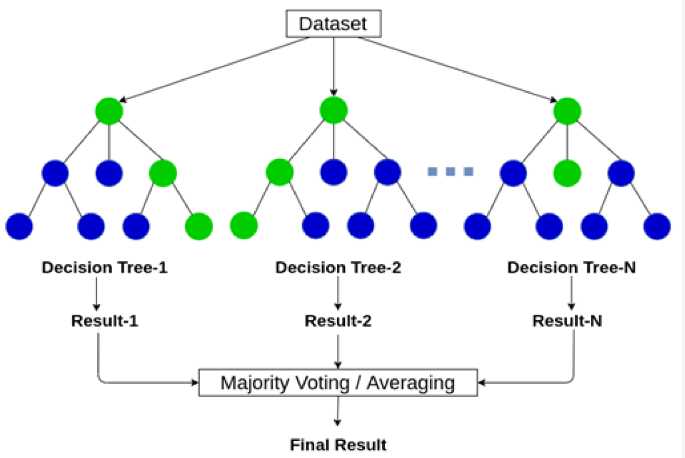
\includegraphics[scale=0.95]{images/random forest regression.png}\\
	\begin{footnotesize}
		\caption{Diagrammatic representation of a random forest \cite{27}}
		\label{Diagrammatic representation of a random forest}
	\end{footnotesize}
\end{figure}

\noindent In this instance, the dataset containing plant images together with the related measures of the number of leaves, leaf area, and fresh weight is used to train the RF regression model. To develop a prediction model, the RF algorithm examines the link between the input attributes (number of leaves and leaf area) and the goal variable (fresh weight). Then, based on the number of leaves and leaf area in the new, unseen plant images, the trained RF model is used to estimate the fresh weight of the plants.
The accuracy and dependability of the biomass estimation are assessed using a variety of measures, including mean squared error, mean absolute error, and R-squared value. In order to verify the model's performance over several subsets of the dataset and reduce overfitting, cross-validation techniques are frequently used.
Overall, by utilizing the variables of leaf area and number of leaves retrieved from plant photos, the RF regression approach plays a significant role in this instance by estimating biomass. It is a useful method for biomass estimation in the context of this study since it can handle non-linear connections, handle high-dimensional data, and give interpretable feature importance analysis.

\subsection{Support Vector Regression}
Support Vector Regression (SVR) is a machine learning algorithm used for biomass estimation based on the attributes of the number of leaves and leaf area extracted from plant images. SVR is a variant of Support Vector Machines (SVM) specifically designed for regression tasks.
In a high-dimensional feature space, SVR seeks to identify a hyperplane that best reflects the relationship between the input attributes (number of leaves and leaf area) and the output variable (Weight). As shown in Figure \ref{Support Vector Regression}, SVR focuses on establishing a hyperplane that achieves a particular degree of precision, known as the margin, around the training samples, as opposed to conventional regression techniques that seek to reduce the errors between the predicted and actual values. When dealing with non-linear correlations between the attributes and the target variable, SVR is especially helpful.
The SVR algorithm converts the input attributes into a higher-dimensional space, where the hyperplane is generated, using a kernel function. SVR is capable to detect complicated correlations and non-linear patterns between leaf area, leaf number, and fresh weight as a result of this change. The qualities of the data and the issue at hand determine whether kernel function, such as linear, polynomial, or radial basis function (RBF), should be used.

\noindent The SVR model is used to estimate the biomass of new plant images based on their number of leaves and leaf area once it has been trained on the dataset comprising plant images and their related biomass. The SVR method predicts the appropriate biomass by applying the learned hyperplane to the input attributes.
In order to evaluate the accuracy and reliability of the biomass estimation, the performance of the SVR model is measured using metrics like mean squared error and R-squared value.
SVR also has the benefit of illuminating the significance of the input features in establishing biomass. Each attribute's contribution to the biomass estimation process can be evaluated by looking at the coefficients or weights corresponding to it. The relationship between the number of leaves, the size of the leaves, and the fresh weight can be better understood with the use of this information.
In summary, Support Vector Regression (SVR) is an effective method used in this case to estimate biomass based on the attributes of the number of leaves and leaf area derived from plant photos. A useful tool for biomass estimation, it can handle high-dimensional data, capture non-linear correlations, and give interpretability via support vectors. SVR aids in revealing intricate patterns and connections between input qualities and fresh weight, enhancing comprehension and decision-making in plant growth, yield prediction, and agricultural management.

\begin{figure}[h]
\centering
	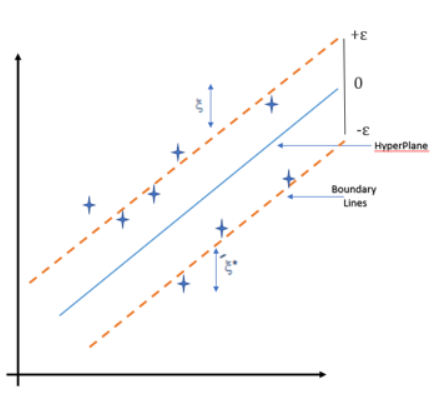
\includegraphics[scale=0.95]{images/svr.png}\\
	\begin{footnotesize}
		\caption{Support Vector Regression \cite{28}}
		\label{Support Vector Regression}
	\end{footnotesize}
\end{figure}

\begin{enumerate}
    \item \textbf{Hyperplane}: It is a boundary separating two data classes in a dimension higher than the actual dimension. It is described in SVR as the line that helps in estimating the desired value.
    
    \item \textbf{Kernel}: In SVR, a higher dimension is utilized for the regression. In order to accomplish that, we require a function that should map the data points into the higher dimension. This function is termed kernel. SVR uses several kernel types, such as Sigmoidal Kernels, Polynomial Kernels, Gaussian Kernels, etc.
    
    \item \textbf{Boundary Lines}: These are the two lines that are drawn at a distance of $varepsilon$ (epsilon) around the hyperplane. It serves as a buffer between the data points.
    
    \item \textbf{Support Vector}: The extreme data points in the dataset that aid in creating the hyperplane are the vector that is utilized to define the hyperplane, or we may say that they are the vector itself.
\end{enumerate}

\subsection{ Multilayer Perceptron}
A popular artificial neural network design called a multilayer perceptron (MLP) is used to estimate the biomass of plants based on the properties of leaf area and leaf number that are derived from plant images. MLP is a feedforward neural network model made up of many interconnected artificial neurons or nodes arranged in layers as shown in Figure \ref{MLP architecture}.
The output variable (biomass) and the input qualities (number of leaves and leaf area) are recognized as complicated non-linear relationships, and MLP is known for its ability to capture these interactions. It is particularly useful in situations where the qualities' intricate connections with the target variables make it difficult to represent them using conventional linear regression methods.
An input layer, one or more hidden layers, and an output layer make up the MLP architecture. Multiple neurons make up each layer, which executes calculations on the incoming data and relay the results to the following layer. Weights are connected to the connections between the neurons, and they are changed throughout training to improve the effectiveness of the network.
By minimizing a predetermined loss function, such as mean squared error or mean absolute error, which measures the difference between the anticipated and actual values throughout the training phase, the MLP model learns which weights are optimal. 

\begin{figure}[h]
\centering
	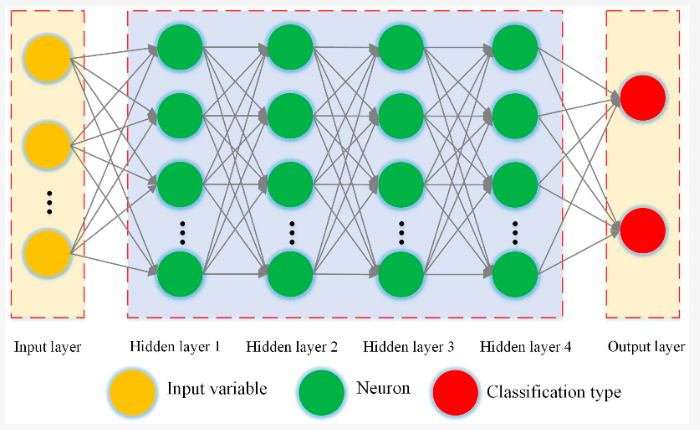
\includegraphics[scale=0.95]{images/mlp.png}\\
	\begin{footnotesize}
		\caption{MLP architecture \cite{29}}
		\label{MLP architecture}
	\end{footnotesize}
\end{figure}

\noindent This model is used to estimate the biomass of new plants based on their number of leaves and leaf area once it has been trained on the dataset comprising plant images and their related fresh weight. The forward pass of the MLP model produces the final output prediction as the input attributes spread through the network, activating the neurons.
The accuracy and predictive capability of the biomass estimation are evaluated using a variety of measures, such as mean squared error, mean absolute error, and R-squared value. In order to evaluate the model's performance over several subsets of the dataset and guarantee its generalizability, cross-validation techniques is also used.
It has a number of benefits for problems involving biomass estimation. Large and varied datasets can be used to generate learning from complex non-linear relationships. Due to MLP's great degree of flexibility, its modeling ability can be improved by adding more hidden layers, neurons, or activation functions. Additionally, MLP can handle high-dimensional data, making it appropriate for situations where the biomass estimating process depends on a number of factors.
In conclusion, Multilayer Perceptron (MLP) is an effective neural network architecture that is employed in this instance to estimate biomass based on the attributes of the number of leaves and leaf area derived from plant images. It is a useful tool for precise biomass estimation because of its capacity to model intricate non-linear interactions and learn from various datasets. MLP assists in analyzing plant growth, forecasting yields, and making agricultural decisions by enhancing our knowledge of the correlations between input variables and fresh weight.

\subsection{k-Nearest Neighbors}
k-Nearest Neighbors (k-NN) is a popular non-parametric machine learning algorithm used for biomass estimation based on the attributes of the number of leaves and leaf area extracted from plant images. k-NN is a simple yet effective algorithm that operates on the principle of similarity and makes predictions based on the characteristics of the k nearest neighbors in the training dataset.
The training dataset, which comprises of plant images together with the associated biomass, is first stored by the k-NN method. When a fresh plant image is given during the prediction phase, the algorithm looks for the k nearest neighbors in the training dataset based on how similar their attributes like leaf area and number of leaves are.
Typically, distance metrics like Euclidean distance or Manhattan distance are used to calculate how similar two plant images are to one another. The characteristics of the new plant image and the attributes of the k nearest neighbors are measured using the k-NN technique. The predicted biomass of the new plant image is determined by aggregating the biomass of the k nearest neighbors, typically through averaging or weighted averaging.

\noindent The k-NN algorithm's performance is influenced by the choice of the parameter k, which represents the number of neighbors to take into account. While a bigger number of k takes into account a wider range of neighbors, a smaller value of k tends to produce more focused predictions. 
simplicity and ease of use in implementation are the benefits of using this algorithm. It can adapt to various data types and makes no assumptions about the distribution of the underlying data. K-NN is also tolerant of outliers and can handle multi-modal data.
The k-NN algorithm does, however, have a few drawbacks. The prediction time can drastically increase as the training dataset gets larger since finding the closest neighbors is necessary. The choice of distance measure and the scale of the input attributes may also have an impact on the way the k-NN algorithm performs. To address these problems, feature scaling is utilized.
In conclusion, the k-Nearest Neighbors (k-NN) technique, which was employed in this instance to estimate biomass based on the attributes of the number of leaves and leaf area derived from plant images, is simple and efficient. K-NN offers predictions for the fresh weight of fresh plants by taking into consideration the traits of the closest neighbors in the training dataset. It is an effective tool for biomass estimation as to its simplicity, adaptability, and capability to handle multi-modal data. Figure \ref{KNN algorithm} shows visual representation of the working of KNN algorithm. 

\begin{figure}[h]
\centering
	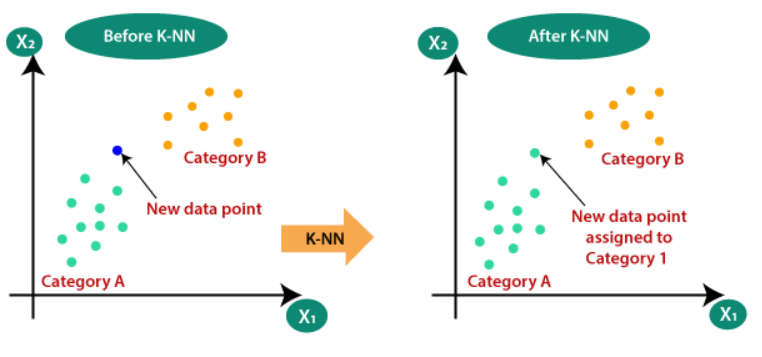
\includegraphics[scale=0.95]{images/knn.png}\\
	\begin{footnotesize}
		\caption{KNN algorithm \cite{30}}
		\label{KNN algorithm}
	\end{footnotesize}
\end{figure}

\section{Hyperparameter tuning}
In order to maximize the performance of machine learning models, hyperparameter tuning is an essential phase in the modeling process. It entails looking for the optimal set of hyperparameters, or parameters that are chosen at the beginning of model training rather than ones that are learned from the data. GridSearchCV is a well-known method for hyperparameter tuning that cross-validates the model's performance while methodically examining a predetermined grid of hyperparameter values.
In our case, we apply hyperparameter tuning using GridSearchCV to fine-tune the Random Forest (RF), Multilayer Perceptron (MLP), Support Vector Machine (SVM), and k-Nearest Neighbors (k-NN) models for biomass estimation based on the number of leaves and leaf area attributes extracted from plant images.

\noindent A collection of hyperparameters are specified for each model, and their associated values are to be investigated. Different combinations of values for each hyperparameter are specified to create the grid of hyperparameters. Following are the hyperparameters taken into account for each model:
% \begin{itemize}
%     \item \textbf{Random Forest}
%     \begin{itemize}
%         \item n\_estimators: the number of trees in the forest
%         \item max\_depth: the maximum depth of each tree
%         \item min\_samples\_split: the minimum number of samples required to split an internal node 
%         \item min\_samples\_leaf: the minimum number of samples required to be at a leaf node
%     \end{itemize}
% \end{itemize}
% \begin{itemize}
%     \item \textbf{Multilayer Perceptron}
%     \begin{itemize}
%         \item hidden\_layer\_sizes: the number of neurons in each hidden layer
%         \item activation: the activation function for the hidden layers
%         \item solver: the optimization algorithm 
%         \item learning\_rate: the learning rate schedule
%     \end{itemize}
% \end{itemize}
% \begin{itemize}
%     \item \textbf{Support Vector Regression}
%     \begin{itemize}
%         \item C: the regularization parameter
%         \item kernel: the kernel function used for mapping the input data to higher-dimensional space
%         \item gamma: the kernel coefficient (for non-linear kernels)
%     \end{itemize}
% \end{itemize}
% \begin{itemize}
%     \item \textbf{k-Nearest Neighbors}
%     \begin{itemize}
%         \item n\_neighbors: the number of neighbors to consider
%         \item weights: the weight function used in prediction
%         \item algorithm: the algorithm used to compute the nearest neighbors
%     \end{itemize}
% \end{itemize}

\subsection{Random Forest}

\begin{figure}[h]
\centering
	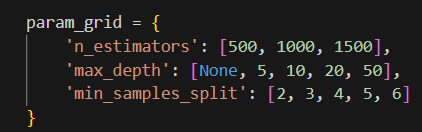
\includegraphics[scale=0.95]{images/rf param.png}\\
	\begin{footnotesize}
		\caption{Random forest parameters}
		\label{Random forest parameters}
	\end{footnotesize}
\end{figure}

\noindent The code snippet in Figure \ref{Random forest parameters} presents a parameter grid that contains a list of hyperparameters for altering a machine learning model, particularly a RandomForest model. These hyperparameters are critical in determining how the model behaves and performs. With values of 500, 1000, and 1500, the "n\_estimators hyperparameter" regulates the number of decision trees included in the RandomForest ensemble, affecting the resilience and complexity of the model.
The "max\_depth" hyperparameter controls the maximum depth of each tree. It provides options such as no depth limit (None) or limited depths of 5, 10, 20, and 50, which affects the tree's ability to capture complicated relationships. With values of 2, 3, 4, 5, and 6, the "min\_samples\_split" hyperparameter controls the minimum number of samples required to split a node, which influences the degree to which the tree is split. 
The code determines the ideal configuration that produces the maximum predictive accuracy and generalization capabilities by methodically testing the model's performance across numerous combinations of these hyperparameters. The improvement of the model's capacity to precisely estimate biomass or make predictions in a wider context depends on this process of hyperparameter tuning.

\subsection{Support Vector Regression}

\begin{figure}[h]
\centering
	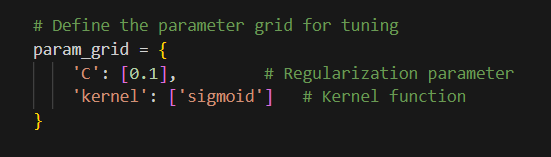
\includegraphics[scale=0.95]{images/svr param.png}\\
	\begin{footnotesize}
		\caption{SVR parameters}
		\label{SVR parameters}
	\end{footnotesize}
\end{figure}

\noindent The above code snippet in Figure \cite{SVR parameters} is a structured arrangement for fine-tuning an SVM model which has a big impact on its performance and behavior. The "C" parameter, which denotes regularization strength, is set to a single value of 100000 here, which affects the trade-off between increasing the margin of the decision border and reducing classification errors.
The "kernel" parameter determines the kind of kernel function that will be utilized in the SVM, and the kernel function 'rbf'(Radial basis function) has been selected to allow for the effective transformation of input data into a higher-dimensional space.
The script determines the most effective configuration that produces the most precise and reliable predictions for tasks like biomass estimation by methodically testing the model's performance across these set parameter combinations.

\subsection{Multilayer Perceptron}

\begin{figure}[h]
\centering
	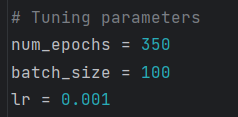
\includegraphics[scale=0.95]{images/mlp param.png}\\
	\begin{footnotesize}
		\caption{MLP parameters}
		\label{MLP parameters}
	\end{footnotesize}
\end{figure}

\noindent The specified hyperparameters in this grid as seen in figure \ref{MLP parameters} have a considerable impact on the MLP's performance. The "hidden\_layer\_sizes" analyzes various hidden layer architectural combinations, influencing the network's ability to learn complex patterns. These possibilities include single layers of 64 and 128 neurons as well as combinations like (64, 32) and (128, 64).
The "activation" parameter offers a choice between 'relu' and 'logistic' activation functions, affecting how information flows through the neural network's nodes.
The "max\_iter" parameter regulates the maximum number of iterations during training, enabling variations of 500, 1000, and 1500 iterations and affecting the network's convergence.

\subsection{k-Nearest Neighbors}

\begin{figure}[h]
\centering
	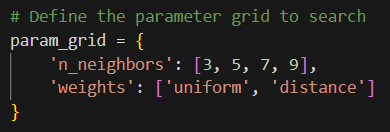
\includegraphics[scale=0.95]{images/knn param.png}\\
	\begin{footnotesize}
		\caption{KNN parameters}
		\label{KNN parameters}
	\end{footnotesize}
\end{figure}

\noindent As seen in Figure \ref{KNN parameters}, the "n\_neighbors" parameter specifies a range of values, including 3, 5, 7, and 9, to indicate how many of the nearest neighbors will be taken into consideration when performing regression tasks. It has an immediate impact on the model's sensitivity to local patterns and the resolution of its decision bounds. 'Uniform' and 'Distance' are the two options for the "weights" parameter that control how nearby data points influence predictions. 



\bigskip
\bigskip


\noindent The GridSearchCV approach orchestrates a thorough exploration by cross-validating the model during training across various permutations of these hyperparameters after specifying the hyperparameters and their corresponding values. This cross-validation strategy reduces overfitting and provides information on how the model performs in hypothetical data scenarios. GridSearchCV uses a specified scoring metric, such as mean squared error or the R-squared value, to evaluate the effectiveness of each collection of hyperparameters. Based on the set of hyperparameters that produces the best performance, the best configuration is chosen.
Using the available features through hyperparameter tuning rendered possible by GridSearchCV, the goal of this research is to identify hyperparameter configurations for biomass estimation that display the best accuracy and robust generalization capabilities. This method improves model performance by identifying configurations that best fit our particular situation. After hyperparameter tweaking, models with the best hyperparameters are evaluated.

\noindent In order to optimize models for biomass estimation such as Random Forest, Multilayer Perceptron, Support Vector Machine, and k-Nearest Neighbors, GridSearchCV is used to carefully tune the hyperparameters. key settings that result in accurate and flexible models are identified the systematic analysis of hyperparameter combinations and rigorous performance evaluation. This approach enhances the predictive power of the model through the use of the given factors, enabling more accurate biomass prediction.

\chapter{Result}
In this section, the results of the investigation into biomass prediction using various machine learning models, namely Random Forest (RF), Support Vector Machine (SVM), Multilayer Perceptron (MLP), and k-Nearest Neighbors (k-NN), are presented. The central focus of this study is to develop a model that precisely estimates biomass utilizing plant phenotypic information. By employing a rigorous methodology and conducting extensive evaluations, valuable knowledge regarding the relative merits of these models is gained, ultimately guiding optimal biomass predictions in the context of plant phenotyping and machine learning.


\noindent The provided graph illustrates a scatter plot depicting the relationship between predicted and actual biomass values, utilizing the dataset and hyperparameters as described earlier. Essential metrics such as the coefficient of determination (r squared), mean squared error (MSE), and mean absolute error (MAE) are incorporated, serving as quantitative indicators for the performance evaluation of each model. The performance metrics are vital in evaluating the accuracy and stability of the models. A thorough analysis of data points and their linked metrics leads to a deep appreciation of the model's predictive powers. The selection of the optimal model, most suitable for the intended purpose of biomass estimation through plant phenotyping and machine learning, can be facilitated through a thorough examination of this graphical and numerical representation.

\section{Scatter plot}

\begin{figure}[ht]
    \centering
    \fbox{
    \begin{minipage}{1.0\textwidth}
        \centering
        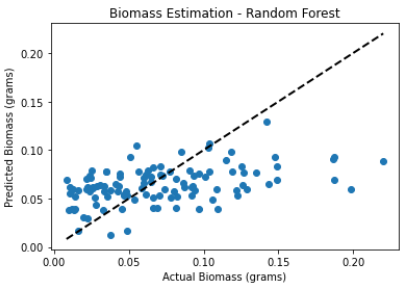
\includegraphics[width=0.45\linewidth]{images/rf output.png} \hfill
        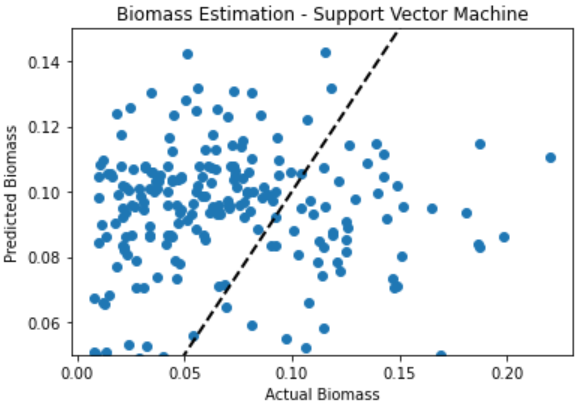
\includegraphics[width=0.45\linewidth]{images/svm output.png} \\
        \vspace{0.5cm}
        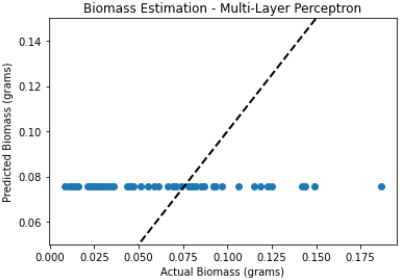
\includegraphics[width=0.45\linewidth]{images/mlp output.png} \hfill
        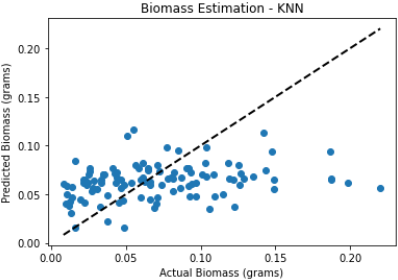
\includegraphics[width=0.45\linewidth]{images/knn output.png}
    \end{minipage}
    }
    \caption{Scatter plots}
    \label{Scatter plots}
\end{figure}

The visualizations in Figure \ref{Scatter plots} depict scatter plots, which serve as a graphical tool for evaluating machine learning models. In these plots, each data point stands in for an observation from the dataset, exhibiting the actual biomass value situated alongside the projected biomass value. The closer points are to the diagonal line, as indicated by the equation "y = x", highlights the accuracy of the predicted values.
Visualizing the relationship between two variables using a scatter plot helps assess the model's accuracy. A clustering of points along the diagonal implies extraordinary accuracy, due to the accurate predictions matching the actual values. If the points are located at a great distance from the diagonal, it implies that the predictions differ considerably from the true values, implying a less reliable model.
As shown on the scatter plot, 'k--' denotes the reference line where perfect predictions align. When the predicted and actual biomass values match, this point will be located at those precise intervals. Any points located nearby or on this line indicate remarkable model effectiveness.

\noindent The code fragment highlighted here plots scatter points by utilizing `y\_test` as the actual values and `y\_pred` as the forecasted values. Using the minimum and maximum values of `y\_test`, the `plt.plot()` function creates a diagonal reference line, which serves as a reference point for evaluation.
In summary, scatter plots visually summarize how well the machine learning models predict biomass values. Intuitive graphical representations are provided, allowing users to gain insight into where and why predictions may be incorrect. A diagonal reference line provides a helpful indicator for assessing the preciseness of forecasts, expediting the evaluation of the model's effectiveness.


\section{Performance metrics}

\begin{table}[h!]
\centering
\begin{tabular}{|c|c|c|c|} 
\hline
Model  & $R^2$ & MSE & MAE \\ 
\hline
Random Forest Regressor  (RF) & 0.171 & 0.002 & 0.033\\
Support Vector Machin  (SVM) & -0.399 & 0.003 & 0.047\\
Multilayer Perceptron (MLP), & -0.104 & 0.002 & 0.036\\
k-Nearest Neighbors (k-NN) & 0.031 & 0.002 & 0.002\\
\hline
\end{tabular}
\caption{Performance metrics result}
\label{table:metrics}
\end{table}

The provided table \ref{table:metrics} is a thorough compilation of the key performance metrics, including Mean Squared Error (MSE), R-squared (R2) value, and Mean Absolute Error (MAE), that are crucial indicators for assessing the accuracy of the machine learning models used in this research study. These metrics collectively illuminate the models' predictive capabilities and their accuracy in estimating biomass values.

\noindent The best-performing hyperparameters for the Random Forest (RF) model, which were carefully selected through the model tuning process, are listed as follows: Max depth is 5, minimum sample split is 6, and there are 1500 estimators. The R2 Score, which gauges how well the model's predictions match actual values, is recorded as being 0.171. The average squared difference between the predicted and actual values is represented by the estimated Mean Squared Error, which is slightly low at 0.002. The Mean Absolute Error, which measures the average magnitude of the mistakes, is also a bit low at 0.033.

\noindent In contrast, the Support Vector Machine (SVM) model exhibits different dynamics. The model's ideal hyperparameters, which were obtained by meticulous tuning, are denoted by the values "C": 100000 and "kernel": "rbf". Even though it is slightly negative at -0.399, the R2 Score illustrates how insufficiently the model captures the data's variation, which is due to the lack of an extensive dataset. The Mean Squared Error, which measures the average squared variances between forecasts and actual values, is 0.003, while the Mean Absolute Error is calculated at 0.047, both of which indicate a moderate level of accuracy.

\noindent Similarly, the Multilayer Perceptron (MLP) model exhibits unique outcomes. For this model, the following hyperparameters were chosen: "activation": "logistic," "hidden\_layer\_sizes": (64, 32)," and "max\_iter": 500. The R2 Score, however, is particularly low, showing subpar performance in terms of predicting the biomass values, which is again as seen previously is due to a small dataset. Calculated as 0.002 and 0.036, respectively, are the Mean Squared Error and Mean Absolute Error.

\noindent Finally, GridSearchCV with cross-validation was used to optimize the k-Nearest Neighbors (k-NN) model, producing the optimum hyperparameters "n\_neighbors": 9 and "weights": "uniform". The observed R2 Score, which represents the percentage of variance in the dependent variable that the model is able to account for, is 0.031. Similar to the other models, the Mean Squared Error is determined to be 0.002, and the Mean Absolute Error has a value of 0.02.

\noindent In summary, this thorough evaluation of the machine learning models, based on the important metrics of MSE, R2 value, and MAE, provides insightful information about the models' propensity for prediction and relative accuracy in estimating biomass levels. The observed performance differences between different models highlight the importance of hyperparameter optimization and model selection in attaining the best results.


\section{Result comparison}
The comparison of the outcomes from different machine learning models offers insightful information regarding the accuracy with which they predict biomass estimation based on plant phenotypic features mentioned above. The Random Forest algorithm showed the most promising results among the models tested. It attained a noteworthy R2 Score of 0.171 with optimized hyperparameters ("max\_depth": 5, "min\_samples\_split": 6, "n\_estimators": 1500), demonstrating a significant connection between predicted and real biomass levels. The model's precision was further highlighted by the exceptionally low Mean Squared Error (MSE) of 0.002 and Mean Absolute Error (MAE) of 0.033.
The Support Vector Machine (SVM) model, on the other hand, showed less promising outcomes, with a negative R2 Score of -0.399, indicating that its predictions significantly deviated from the observed values. In comparison to the Random Forest model, the corresponding MSE and MAE values were also noticeably higher, indicating decreased accuracy. The Multilayer Perceptron (MLP) model's performance was also hampered by its poor R2 Score of -0.104, which indicates a lackluster capacity for prediction. The MLP model's calculated MSE and MAE values provided more evidence of its shortcomings in terms of precise biomass calculation.
With an R2 Score of 0.031, the k-Nearest Neighbors (k-NN) model performed mediocrely. Although it performed somewhat better than the SVM and MLP models, it was still less accurate than the Random Forest model.

\noindent It is noteworthy that the SVM, MLP, and k-NN models' subpar performance could be attributable to the limited dataset size of 530 samples. Larger datasets are frequently necessary for machine learning algorithms to properly identify significant patterns and correlations. The little dataset in this research might have hindered the models' ability to generalize and produce precise predictions, especially for the intricate correlations between phenotypic variables and biomass. As a result, the Random Forest model performed better because to its superiority in managing such complexity and its ability to identify complicated patterns in the data. This demonstrates how important dataset quantity and quality are for building reliable and precise machine learning models to predict biomass.


\chapter{Conclusion}
In conclusion, this study aims to apply machine learning to estimate biomass through the examination of phenotypic features in plants. In order to effectively forecast biomass, the study concentrated on using advanced algorithms including Random Forest, Support Vector Machine, Multilayer Perceptron, and k-Nearest Neighbors. The research started with the gathering of a diverse dataset, which included carefully cultivated plants in a controlled glasshouse environment.
Preprocessing techniques were meticulously used to reduce noise and irregularities in the dataset. Following that, feature extraction techniques were used, identifying leaf area and count as essential attributes. The study examined contour analysis, picture segmentation, shape descriptors, and texture analysis as tools to extract these features effectively.
The retrieved features served as the foundation for the input variables for the models, namely leaf area and leaf count. The algorithms were calibrated to predict Weight, a key biomass metric, using a thorough training and evaluation process. The study included a thorough evaluation of model performance, hyperparameter optimization, and the application of cross-validation methods. To measure prediction accuracy, evaluation metrics like R2 Score, Mean Squared Error (MSE), and Mean Absolute Error (MAE) were computed.

\noindent In the realm of results, the Random Forest model emerged as the frontrunner with R2 value of 0.171 and minimal MSE and MAE. This achievement highlighted the model's skill at capturing complex correlations in the data. However, due in part to the limited dataset size, the Support Vector Machine, Multilayer Perceptron, and k-Nearest Neighbors models produced very modest results.
It is imperative to emphasize the value of reliable data in determining the research's conclusions. A comprehensive and reliable dataset fortifies the accuracy and reliability of machine learning models, especially when tackling complex tasks such as estimating biomass.

\noindent In summation, this research emphasizes the potential of machine learning in biomass prediction and also highlights the importance of model choice and dataset quality. We are moving toward a future where plant phenotypic features and cutting-edge algorithms work together to change biomass estimation techniques, enabling more accurate decisions in agriculture, ecology, and other fields thanks to the predominance of the Random Forest model, which is supported by rigorous evaluation.


\chapter{Future scope}
Future scope in this field has an immense amount of potential to increase our understanding of how to estimate biomass in plants using phenotypic features and machine learning. The interesting opportunities for expanding this study are outlined in the following major points:
\begin{itemize}
    \item \textbf{Enhancement of Dataset:} The dataset should be diversified and expanded as a top priority. More reliable and generalizable models will result from the collection of data from a greater variety of plant species, growth stages, and environmental circumstances. To assemble a comprehensive dataset, efforts can be focused on partnering with botanical gardens, academic organizations, and farming operations.

    \item \textbf{Utilization of High-Quality Cameras:} Images of plants that are clearer and more detailed can be produced by integrating new imaging technologies that have better resolutions and improved spectrum capabilities. As a result, feature extraction will be of higher quality, and biomass prediction will be more accurate.

    \item \textbf{Deep Learning and Neural Networks:} Convolutional neural networks (CNNs), in particular, can be used to combine deep learning approaches to automatically extract features from images. Increased predictive power is possible with transfer learning, which involves optimizing pre-trained models for biomass estimation.

    \item \textbf{Generalization of Models:} It is essential to adjust the created models to account for various plant types and phenotypic deviations. Research efforts can concentrate on developing more adaptable models that can precisely estimate biomass across various plant species and growing conditions.

    \item \textbf{Real-Time Monitoring and UAV Integration:} Precision agriculture can be revolutionized by expanding the research to include real-time biomass estimation using Unmanned Aerial Vehicles (UAVs) and ground-based imaging systems. To make fast decisions and manage resources, automated data gathering and ongoing plant growth monitoring will be used.

    \item \textbf{Integration of Environmental Factors:} The prediction accuracy of the models can be improved by including environmental factors like temperature, humidity, and light intensity as input features. The elements affecting biomass accumulation may be better understood with the help of this comprehensive approach.

    \item \textbf{Integration with IoT and Sensor Networks:} Continuous and automated monitoring of plant phenotypic features can be made possible by utilizing Internet of Things (IoT) devices and sensor networks for data collecting. This connection could potentially make the biomass estimating process more dynamic and flexible.

    \item \textbf{Commercial and Agricultural Applications:} Collaborating with farmers and agricultural technology businesses can help turn research findings into useful tools and solutions. The creation of user-friendly software, mobile applications, or cloud-based platforms can increase the accessibility and usefulness of biomass estimation to a larger audience.
\end{itemize}

\noindent In summary, the research's future directions include a comprehensive strategy for improving data collecting, developing more complex models, extending the range of applications, and bridging the gap between academia and industry. The combination of these efforts has the potential for transforming plant phenotyping and biomass estimation, advancing ecological research and sustainable agriculture.














































































\newpage
\listoffigures\addcontentsline{toc}{chapter}{List of Figures}
\newpage
\listoftables\addcontentsline{toc}{chapter}{List of Tables}






\newpage
\begin{thebibliography}{1}\markboth{Bibliography}{Bibliography}\addcontentsline{toc}{chapter}{Bibliography}

% %for a article
% \bibitem{1}
% Bundesverband der Energie- und Wasserwirtschaft e.V (BDEW) (2022). Entwicklung des Wärmeverbrauchs in Deutschland: Basisdaten und Einflussfaktoren

 %for a article
\bibitem{1}
https://www.electronicwings.com/users/dhruvshethlinkit/projects/1628/plant-growth-estimation-for-high-throughput-phenotyping

\bibitem{2}
Christine Granier, Denis Vile,
Phenotyping and beyond: modelling the relationships between traits,
Current Opinion in Plant Biology,
Volume 18,
2014,
Pages 96-102,
ISSN 1369-5266,
https://doi.org/10.1016/j.pbi.2014.02.009.

\bibitem{3}
Rahaman MM, Ahsan MA, Gillani Z, Chen M. Digital Biomass Accumulation Using High-Throughput Plant Phenotype Data Analysis. J Integr Bioinform. 2017 Sep 1;14(3):20170028. doi: 10.1515/jib-2017-0028. PMID: 28862986; PMCID: PMC6042821.

\bibitem{4}
Ali, Jehad \& Khan, Rehanullah \& Ahmad, Nasir \& Maqsood, Imran. (2012). Random Forests and Decision Trees. International Journal of Computer Science Issues(IJCSI). 9. 

\bibitem{5}
Basak, Debasish \& Pal, Srimanta \& Patranabis, Dipak. (2007). Support Vector Regression. Neural Information Processing – Letters and Reviews. 11. 

\bibitem{6}
Nazzal, Jamal \& El-Emary, Ibrahim \& Najim, Salam. (2008). Multilayer Perceptron Neural Network (MLPs) For Analyzing the Properties of Jordan Oil Shale. World Applied Sciences Journal. 5. 

\bibitem{7}
Yao, Z., Ruzzo, W.L. A Regression-based K nearest neighbor algorithm for gene function prediction from heterogeneous data. BMC Bioinformatics 7 (Suppl 1), S11 (2006). https://doi.org/10.1186/1471-2105-7-S1-S11

\bibitem{8}
Lee U, Chang S, Putra GA, Kim H, Kim DH (2018) An automated, high-throughput plant phenotyping system using machine learning-based plant segmentation and image analysis. PLOS ONE 13(4): e0196615. https://doi.org/10.1371/journal.pone.0196615

\bibitem{9}
https://www.fsm.ac.in/blog/an-introduction-to-machine-learning-its-importance-types-and-applications/

\bibitem{10}
Alzubaidi, L., Zhang, J., Humaidi, A.J. et al. Review of deep learning: concepts, CNN architectures, challenges, applications, future directions. J Big Data 8, 53 (2021). https://doi.org/10.1186/s40537-021-00444-8

\bibitem{11}
Roza Dastres, Mohsen Soori. Artificial Neural Network Systems. International Journal of Imaging
and Robotics (IJIR), 2021, 21 (2), pp.13-25. ffhal-03349542f

\bibitem{12}
https://www.analyticsvidhya.com/blog/2021/04/beginners-guide-to-explanatory-data-analysis/

\bibitem{13}
https://askdatascience.com/13/what-are-the-main-branches-of-machine-learning

\bibitem{14}
https://astrobotany.com/arabidopsis/

\bibitem{15}
Tran, Hai \& Triet, L.M. \& Le, Thai \& Thuy, N.T.. (2017). Real Time Burning Image Classification Using Support Vector Machine. EAI Endorsed Transactions on Context-aware Systems and Applications. 4. 152760. 10.4108/eai.6-7-2017.152760. 

\bibitem{16}
https://www.analyticsvidhya.com/blog/2020/11/hyperparameter-tuning-using-optuna/

\bibitem{17}
https://www.geeksforgeeks.org/underfitting-and-overfitting-in-machine-learning/

\bibitem{18}
Cioffi, \& Travaglioni, Marta \& Piscitelli, \& Petrillo, Antonella \& Felice, De. (2020). Artificial Intelligence and Machine Learning Applications in Smart Production: Progress, Trends, and Directions. Sustainability. 12. 492. 10.3390/su12020492.

\bibitem{19}
Niklas Kühl, Marc Goutier, Robin Hirt, Gerhard Satzger. Machine Learning in Artificial Intelligence: Towards a Common Understanding. 
https://doi.org/10.48550/arXiv.2004.04686

\bibitem{20}
M. S. B. M. M. P. W. (2014). Research Paper on Basic of Artificial Neural Network. International Journal on Recent and Innovation Trends in Computing and Communication, 2(1), 96–100. https://doi.org/10.17762/ijritcc.v2i1.2920

\bibitem{21}
https://www.ibm.com/topics/neural-networks/

\bibitem{22}
Sarker, I.H. Machine Learning: Algorithms, Real-World Applications and Research Directions. SN COMPUT. SCI. 2, 160 (2021). https://doi.org/10.1007/s42979-021-00592-x

\bibitem{23}
https://www.ncl.ac.uk/webtemplate/ask-assets/external/maths-resources/statistics/regression-and-correlation/coefficient-of-determination-r-squared.html

\bibitem{24}
https://vitalflux.com/r-squared-explained-machine-learning/

\bibitem{25}
https://www.britannica.com/science/mean-squared-error

\bibitem{26}
https://emilia-orellana44.medium.com/not-nice-square-error-2d18c248391c

\bibitem{27}
Hao, L.; Kim, J.; Kwon, S.; Ha, I.D. Deep Learning-Based Survival Analysis for High-Dimensional Survival Data. Mathematics 2021, 9, 1244. https://doi.org/10.3390/math9111244

\bibitem{28}
https://www.educba.com/support-vector-regression/

\bibitem{29}
Jiang, W.; He, G.; Long, T.; Ni, Y.; Liu, H.; Peng, Y.; Lv, K.; Wang, G. Multilayer Perceptron Neural Network for Surface Water Extraction in Landsat 8 OLI Satellite Images. Remote Sens. 2018, 10, 755. https://doi.org/10.3390/rs10050755

\bibitem{30}
https://www.javatpoint.com/k-nearest-neighbor-algorithm-for-machine-learning

\bibitem{31}
Johnson, Xenie & Bouchez, David. (2007). The Model Species, Arabidopsis thaliana. 10.1201/b10760-23. 

\bibitem{32}
Golzarian, M.R., Frick, R.A., Rajendran, K. et al. Accurate inference of shoot biomass from high-throughput images of cereal plants. Plant Methods 7, 2 (2011). https://doi.org/10.1186/1746-4811-7-2

\bibitem{33}
Dipak Pralhad Mahurkar, Hemant Patidar,
Revealing leaf species through specific contour and region-based features extraction,
e-Prime - Advances in Electrical Engineering, Electronics and Energy,
Volume 5,
2023,
100228,
ISSN 2772-6711,
https://doi.org/10.1016/j.prime.2023.100228.
(https://www.sciencedirect.com/science/article/pii/S2772671123001237)


\bibitem{34}
Wang, Li’ai \& Zhou, Xudong \& Zhu, Xinkai \& Dong, Zhaodi \& Guo, Wenshan. (2016). Estimation of biomass in wheat using random forest regression algorithm and remote sensing data. The Crop Journal. 4. 10.1016/j.cj.2016.01.008.


\bibitem{35}
Biswabiplab Singh1 Sudhir Kumar1 Allimuthu Elangovan1 Devendra Vasht1 Sunny Arya1 Nguyen Trung Duc1,2 Pooja Swami1 Godawari Shivaji Pawar3 Dhandapani Raju1 Hari Krishna4 Lekshmy Sathee1 Monika Dalal5 Rabi Narayan Sahoo6 Viswanathan Chinnusamy1,
Phenomics based prediction of plant biomass and leaf area in wheat using machine learning approaches,
Front. Plant Sci., 28 June 2023
Sec. Technical Advances in Plant Science
Volume 14 - 2023 | https://doi.org/10.3389/fpls.2023.1214801


\bibitem{36}
Liu, Wenjian \& Li, Yanjie \& Liu, Jun \& Jiang, Jingmin. (2021). Estimation of Plant Height and Aboveground Biomass of Toona sinensis under Drought Stress Using RGB-D Imaging. Forests. 12. 10.3390/f12121747. 

\bibitem{37}
Fitsum T Teshome, Haimanote K Bayabil, Gerrit Hoogenboom, Bruce Schaffer, Aditya Singh, Yiannis Ampatzidis,
Unmanned aerial vehicle (UAV) imaging and machine learning applications for plant phenotyping,
Computers and Electronics in Agriculture,
Volume 212,
2023,
108064,
ISSN 0168-1699,
https://doi.org/10.1016/j.compag.2023.108064

\bibitem{38}
Kolisetty, Vishnu \& Rajput, Dharmendra. (2019). A Review on the Significance of Machine Learning for Data Analysis in Big Data. Jordanian Journal of Computers and Information Technology. 06. 1. 10.5455/jjcit.71-1564729835. 

\bibitem{39}
Yao, Fupin. “Machine learning with limited data.” ArXiv abs/2101.11461 (2021): n. pag.

\bibitem{40}
https://assets.publishing.service.gov.uk \\ /government/uploads/system/uploads/attachment\_data/file/941511\\/Machine\_Learning\_with\_Limited\_Data\_original\_version\_.pdf

\bibitem{41}
https://www.statisticshowto.com/absolute-error/

\bibitem{42}
https://ogrisel.github.io/scikit-learn.org/sklearn-tutorial/tutorial/astronomy/general\_concepts.html

\bibitem{43}
Amiri, Roohollah & Mehrpouyan, Hani & Fridman, Lex & Mallik, Ranjan & Nallanathan, Arumugam & Matolak, David. (2018). A Machine Learning Approach for Power Allocation in HetNets Considering QoS. 

\bibitem{43}
https://www.geeksforgeeks.org/underfitting-and-overfitting-in-machine-learning/

\bibitem{44}
https://www.masterschool.com/magazine/data-is-the-new-gold/


\end{thebibliography}
\newpage
\appendix
\end{document}